\documentclass[a4paper, 12pt]{article}
% packages
\usepackage{amssymb}
\usepackage[fleqn]{mathtools}
\usepackage{tikz}
\usepackage{enumerate}
\usepackage{bussproofs}
\usepackage{xcolor}
\usepackage[margin=1.3cm]{geometry}
\usepackage{logicproof}
\usepackage{diagbox}
\usepackage{listings}
\usepackage{graphicx}
\usepackage{lstautogobble}
\usepackage{hyperref}
\usepackage{multirow}
\usepackage{tipa}
\usetikzlibrary{decorations.pathreplacing, arrows, shapes.gates.logic.US, circuits.logic.US, calc, automata, positioning, intersections}

% shorthand for verbatim
% this clashes with logicproof, so maybe fix this at some point?
\catcode`~=\active
\def~#1~{\texttt{#1}}

% code listing
\lstdefinestyle{main}{
    numberstyle=\tiny,
    breaklines=true,
    showspaces=false,
    showstringspaces=false,
    tabsize=2,
    numbers=left,
    basicstyle=\ttfamily,
    columns=fixed,
    fontadjust=true,
    basewidth=0.5em,
    autogobble,
    xleftmargin=3.0ex,
    mathescape=true
}
\newcommand{\dollar}{\mbox{\textdollar}} %
\lstset{style=main}

% augmented matrix
\makeatletter
\renewcommand*\env@matrix[1][*\c@MaxMatrixCols c]{%
\hskip -\arraycolsep
\let\@ifnextchar\new@ifnextchar
\array{#1}}
\makeatother

% ceiling / floor
\DeclarePairedDelimiter{\ceil}{\lceil}{\rceil}
\DeclarePairedDelimiter{\floor}{\lfloor}{\rfloor}

% custom commands
\newcommand{\indefint}[2]{\int #1 \, \mathrm{d}#2}
\newcommand{\defint}[4]{\int_{#1}^{#2} #3 \, \mathrm{d}#4}
\newcommand{\pdif}[2]{\frac{\partial #1}{\partial #2}}
\newcommand{\dif}[2]{\frac{\mathrm{d}#1}{\mathrm{d}#2}}
\newcommand{\limit}[2]{\raisebox{0.5ex}{\scalebox{0.8}{$\displaystyle{\lim_{#1 \to #2}}$}}}
\newcommand{\summation}[2]{\sum\limits_{#1}^{#2}}
\newcommand{\product}[2]{\prod\limits_{#1}^{#2}}
\newcommand{\intbracket}[3]{\left[#3\right]_{#1}^{#2}}
\newcommand{\ulsmash}[1]{\underline{\smash{#1}}}

\newcommand{\powerset}[0]{\wp}
\renewcommand{\emptyset}[0]{\varnothing}

\makeatletter
\newsavebox{\@brx}
\newcommand{\llangle}[1][]{\savebox{\@brx}{\(\m@th{#1\langle}\)}%
  \mathopen{\copy\@brx\kern-0.5\wd\@brx\usebox{\@brx}}}
\newcommand{\rrangle}[1][]{\savebox{\@brx}{\(\m@th{#1\rangle}\)}%
  \mathclose{\copy\@brx\kern-0.5\wd\@brx\usebox{\@brx}}}
\makeatother
\newcommand{\lla}{\llangle}
\newcommand{\rra}{\rrangle}
\newcommand{\la}{\langle}
\newcommand{\ra}{\rangle}
\newcommand{\crnr}[1]{\text{\textopencorner} #1 \text{\textcorner}}
\newcommand{\laplace}{\mathcal{L}}
\newcommand{\fourier}{\mathcal{F}}

\newcommand{\mat}[1]{\boldsymbol{#1}}
\renewcommand{\vec}[1]{\boldsymbol{#1}}
\newcommand{\rowt}[1]{\begin{bmatrix}
    #1
\end{bmatrix}^\top}

\newcommand{\unaryproof}[2]{\AxiomC{#1} \UnaryInfC{#2} \DisplayProof}
\newcommand{\binaryproof}[3]{\AxiomC{#1} \AxiomC{#2} \BinaryInfC{#3} \DisplayProof}
\newcommand{\trinaryproof}[4]{\AxiomC{#1} \AxiomC{#2} \AxiomC{#3} \TrinaryInfC{#4} \DisplayProof}

\newcommand{\axiom}[1]{\AxiomC{#1}}
\newcommand{\unary}[1]{\UnaryInfC{#1}}
\newcommand{\binary}[1]{\BinaryInfC{#1}}
\newcommand{\trinary}[1]{\TrinaryInfC{#1}}
\newcommand{\quaternary}[1]{\QuaternaryInfC{#1}}
\newcommand{\quinary}[1]{\QuinaryInfC{#1}}
\newcommand{\dproof}[0]{\DisplayProof}

\newcommand{\bnfsep}[0]{\ |\ }
\newcommand{\lrbt}[0]{\ \bullet\ }
\newcommand{\concsep}[0]{\ ||\ }
\newcommand{\ttbs}{\char`\\}

\newcommand{\violet}[1]{\textcolor{violet}{#1}}
\newcommand{\blue}[1]{\textcolor{blue}{#1}}
\newcommand{\red}[1]{\textcolor{red}{#1}}

% no indent
\setlength\parindent{0pt}

% reasoning proofs
\usepackage{ltablex}
\usepackage{environ}
\keepXColumns
\NewEnviron{reasoning}{
    \begin{tabularx}{\textwidth}{rlX}
        \BODY
    \end{tabularx}
}
\newcommand{\proofline}[3]{$(#1)$ & $#2$ & \hfill #3 \medskip \\}
\newcommand{\proofarbitrary}[1]{& take arbitrary $#1$ \medskip \\}
\newcommand{\prooftext}[1]{\multicolumn{3}{l}{#1} \medskip \\}
\newcommand{\proofmath}[3]{$#1$ & = $#2$ & \hfill #3 \medskip \\}
\newcommand{\prooftherefore}[1]{& $\therefore #1$ \medskip \\}
\newcommand{\proofbc}[0]{\prooftext{\textbf{Base Case}}}
\newcommand{\proofis}[0]{\prooftext{\textbf{Inductive Step}}}

% reasoning er diagrams
\newcommand{\nattribute}[4]{
    \node[draw, state, inner sep=0cm, minimum size=0.2cm, label=#3:{#4}] (#1) at (#2) {};
}
\newcommand{\mattribute}[4]{
    \node[draw, state, accepting, inner sep=0cm, minimum size=0.2cm, label=#3:{#4}] (#1) at (#2) {};
}
\newcommand{\dattribute}[4]{
    \node[draw, state, dashed, inner sep=0cm, minimum size=0.2cm, label=#3:{#4}] (#1) at (#2) {};
}
\newcommand{\entity}[3]{
    \node[] (#1-c) at (#2) {#3};
    \node[inner sep=0cm] (#1-l) at ($(#1-c) + (-1, 0)$) {};
    \node[inner sep=0cm] (#1-r) at ($(#1-c) + (1, 0)$) {};
    \node[inner sep=0cm] (#1-u) at ($(#1-c) + (0, 0.5)$) {};
    \node[inner sep=0cm] (#1-d) at ($(#1-c) + (0, -0.5)$) {};
    \draw
    ($(#1-c) + (-1, 0.5)$) -- ($(#1-c) + (1, 0.5)$) -- ($(#1-c) + (1, -0.5)$) -- ($(#1-c) + (-1, -0.5)$) -- cycle;
}
\newcommand{\relationship}[3]{
    \node[] (#1-c) at (#2) {#3};
    \node[inner sep=0cm] (#1-l) at ($(#1-c) + (-1, 0)$) {};
    \node[inner sep=0cm] (#1-r) at ($(#1-c) + (1, 0)$) {};
    \node[inner sep=0cm] (#1-u) at ($(#1-c) + (0, 1)$) {};
    \node[inner sep=0cm] (#1-d) at ($(#1-c) + (0, -1)$) {};
    \draw
    ($(#1-c) + (-1, 0)$) -- ($(#1-c) + (0, 1)$) -- ($(#1-c) + (1, 0)$) -- ($(#1-c) + (0, -1)$) -- cycle;
}

% actual document
\begin{document}
    \section*{CO211 - Operating Systems}
        \subsection*{4th October 2019}
            \subsubsection*{Outline of the Course}
                \begin{itemize}
                    \itemsep0em
                    \item overview and introduction \hfill structure, case studies
                    \item processes and threads \hfill abstractions that an OS uses to execute code
                    \item inter-process communication (IPC) \hfill allows multiple processes to communicate with each other
                    \item memory management \hfill allocation, abstraction for virtual memory, paging
                    \item device management \hfill types, drivers
                    \item disk management \hfill scheduling, caching, RAID
                    \item file systems \hfill basic abstractions for storage and implementation
                    \item security \hfill authentication, access control
                \end{itemize}
                Note that this follows a similar structure to most OS courses, and therefore we can reference content from other sources.
                \textit{Operating Systems: Three Easy Pieces} is recommended, as it bridges between this course and the PintOS lab.
            \subsubsection*{Overview}
                The general overview is that there is a system bus that interconnects different hardware components (including CPU and memory), and allows for communication between them.
                \medskip

                The operating system provides abstractions for programs to use, meaning that they do not have to deal with the complex hardware.
                For example, a process abstraction expects an interface to the hardware, which allows programs to be used on different hardware.
                This means that the OS will need how to to control the hardware with drivers.
                The operating system has the following goals;
                \begin{enumerate}[(1)]
                    \itemsep0em
                    \item \textbf{managing resources}
                        \medskip

                        The operating system must be able to expose the resources efficiently to the application, and also share these resources fairly.
                        Some examples are;
                        \begin{itemize}
                            \itemsep0em
                            \item CPU (multiple cores) \hfill should decide what runs on each hardware thread
                            \item memory \hfill cache, RAM
                            \item I/O devices \hfill displays (GPUs), network interfaces
                            \item internal devices \hfill clocks, timers, interrupt controllers
                            \item persistent storage
                        \end{itemize}
                        OS uses both time and space multiplexing for sharing.
                        An example for the former is how the effect of parallelism can be achieved with a single CPU core by splitting up the time allocated per process, and an example for the latter is splitting up memory for each process.
                        \medskip

                        On the other hand, with allocation, the OS must also support simultaneous resource access (such as to disks, RAM, network etc.).
                        Continuing from this, it must also offer mutual exclusion, thus protecting risky operations (such as file writing).
                        Generally, the OS aims to protect against corruption.
                        \medskip

                        Finally, the operating system must also handle storing data, and enforce access control.
                    \item \textbf{clean interfaces}
                        \medskip

                        The OS should hide away the hardware, and applications use the hardware through an interface provided by the operating system.
                        We can think of this as a virtual machine abstraction on top of the bare machine - similar to how the JVM works (but at a lower layer).
                    \item \textbf{concurrency and non-determinism}
                        \medskip

                        The operating system must be able to deal with concurrency, for example overlapping I/O and computation.
                        This is because I/O devices tend to be slower, and while the device is working on the task, it shouldn't prevent the CPU from doing other work.
                        An operating system may switch activities at arbitrary times, and this must be done safely - by offering synchronisation primitives.
                        It should also protect processes by giving each program its own space, thus preventing interference.
                        \medskip

                        Similarly, the OS is fundamentally non-deterministic, as it needs to handle interrupts (such as the network card receiving a packet, user interrupts, etc.).
                \end{enumerate}
            \subsubsection*{Tutorial Questions}
                \begin{enumerate}[1)]
                    \itemsep0em
                    \item List the most important resources that must be managed by an operating system in the following settings;
                        \begin{enumerate}[(a)]
                            \itemsep0em
                            \item supercomputer
                                \begin{itemize}
                                    \itemsep0em
                                    \item computation time \hfill primarily used for intensive computations
                                    \item memory
                                \end{itemize}
                            \item networked workstations connected to a server
                                \begin{itemize}
                                    \itemsep0em
                                    \item bandwidth \hfill must handle packet processing and network traffic
                                \end{itemize}
                            \item smartphone
                                \begin{itemize}
                                    \itemsep0em
                                    \item energy \hfill limited power, can power off unused hardware
                                    \item mobile network \hfill (including other communication technology)
                                    \item other sensors \hfill issues of privacy, when to expose GPS etc.
                                \end{itemize}
                        \end{enumerate}
                        As this highlights, some uses will need specially designed operating systems.
                        We also have general-process OS, as it takes a large amount of effort to implement a new operating system.
                    \item What is the \textbf{kernel} of an operating system?
                        \medskip

                        The part of the OS is always in memory, and runs in the privileged part of the CPU (user mode cannot access all functionality).
                        Implements commonly used functions of the OS and has complete access to all hardware.
                \end{enumerate}
            \subsubsection*{Kernel Design}
                \begin{itemize}
                    \itemsep0em
                    \item \textbf{monolithic kernel}
                        \medskip

                        Consider it as one large program that has all the functionality that you want an OS to perform.
                        \medskip

                        The kernel is a single executable with its own address space.
                        There exists a \textbf{system call} interface that allows user mode applications to access the hardware.
                        Software invokes functionality from the kernel by issuing system calls - the CPU must switch from user mode to kernel mode to support this.
                        The kernel then executes some instruction on behalf of the application.
                        Device drivers are part of the monolithic kernel.
                        \begin{center}
                            \begin{minipage}[t]{0.45\textwidth}
                                advantages
                                \begin{itemize}
                                    \itemsep0em
                                    \item efficient calls within the kernel, as there it remains in kernel mode
                                    \item flexible to write kernel components due to the shared memory (direct access with no limit to APIs)
                                \end{itemize}
                            \end{minipage}
                            \hfill
                            \begin{minipage}[t]{0.45\textwidth}
                                disadvantages
                                \begin{itemize}
                                    \itemsep0em
                                    \item complex design
                                    \item no protection between bits of kernel functionality, therefore any bugs within the kernel will crash the entire machine
                                \end{itemize}
                            \end{minipage}
                        \end{center}
                    \item \textbf{microkernels}
                        \medskip

                        Only includes functionality that \textbf{requires} direct access to the hardware (or to be run in kernel mode).
                        This is a minimalistic design and has the advantage of fewer bugs (due to the smaller amount of code).
                        \begin{center}
                            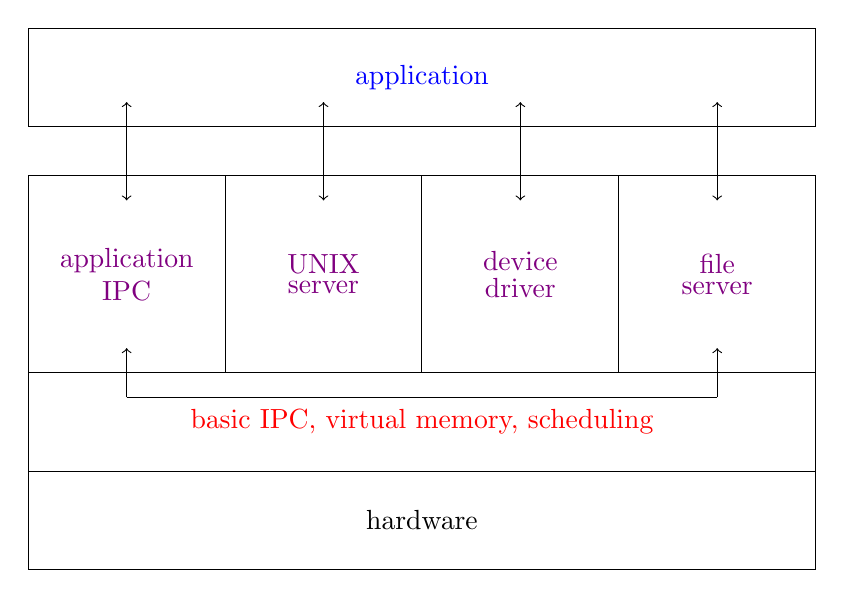
\begin{tikzpicture}[x=2.5cm, y=1.25cm]
                                \node[blue] at (2, -0.5) {application};
                                \node[violet] at (0.5, -2.5) {\shortstack{application\\IPC}};
                                \node[violet] at (1.5, -2.5) {\shortstack{UNIX\\server}};
                                \node[violet] at (2.5, -2.5) {\shortstack{device\\driver}};
                                \node[violet] at (3.5, -2.5) {\shortstack{file\\server}};
                                \node[red] at (2, -4) {basic IPC, virtual memory, scheduling};
                                \node at (2, -5) {hardware};

                                \draw
                                (0.5, -0.75) edge[<->] (0.5, -1.75)
                                (1.5, -0.75) edge[<->] (1.5, -1.75)
                                (2.5, -0.75) edge[<->] (2.5, -1.75)
                                (3.5, -0.75) edge[<->] (3.5, -1.75)
                                (0.5, -3.75) edge[->] (0.5, -3.25)
                                (3.5, -3.75) edge[->] (3.5, -3.25)
                                (0.5, -3.75) -- (3.5, -3.75);

                                \draw (0, 0) -- (4, 0) -- (4, -1) -- (0, -1) -- cycle;
                                \draw (0, -1.5) -- (4, -1.5) -- (4, -3.5) -- (0, -3.5) -- cycle
                                (1, -1.5) -- (1, -3.5)
                                (2, -1.5) -- (2, -3.5)
                                (3, -1.5) -- (3, -3.5);
                                \draw (0, -3.5) -- (0, -4.5) -- (4, -4.5) -- (4, -3.5);
                                \draw (0, -4.5) -- (0, -5.5) -- (4, -5.5) -- (4, -4.5);
                            \end{tikzpicture}
                        \end{center}
                        Note that both the \blue{application} and \violet{servers} run in user mode, and the \red{kernel} is in kernel mode.
                        The kernel performs IPC between the servers, which are separated for device I/O, scheduling. file access etc.
                        \begin{center}
                            \begin{minipage}[t]{0.45\textwidth}
                                advantages
                                \begin{itemize}
                                    \itemsep0em
                                    \item less complex kernel
                                    \item clean interfaces for the servers
                                    \item more reliable; one of the servers could crash and then restart, without bringing the entire kernel down
                                \end{itemize}
                            \end{minipage}
                            \hfill
                            \begin{minipage}[t]{0.45\textwidth}
                                disadvantages
                                \begin{itemize}
                                    \itemsep0em
                                    \item performance overhead due to the requirement of message passing and transitioning between user mode and kernel mode (checks must be done to maintain the separation) - less of an issue now due to better hardware (e.g \textit{Android})
                                \end{itemize}
                            \end{minipage}
                        \end{center}
                    \item \textbf{hybrid kernel} \hfill many modern designs use a combination of both
                        \medskip

                        This is a more structured design, however user-level servers can incur a performance penalty.
                \end{itemize}
            \subsubsection*{Linux Kernel}
                The structure of Linux system calls is to put arguments into registers Or on the stack, and then issue a trap to switch the CPU from user to kernel mode.
                \medskip

                While C is the dominant language for the Linux kernel, the interrupt handlers are written in assembly, as they are low level pieces of code, and require fast performance (hence a low instruction count).
                Interrupt handlers are the primary means to interact with devices, it initiates dispatching which stops proxies, saves the state, starts the driver and returns.
                \medskip

                Typically, we can split the Linux kernel into three parts;
                \begin{itemize}
                    \itemsep0em
                    \item \textbf{I/O}
                        \medskip

                        One of the design philosophies under UNIX style operating system is to treat everything as a file, and use this file abstraction to expose different resources.
                        Therefore, a lot of I/O resources can be hidden under this virtual file system.
                    \item \textbf{memory management}
                        \medskip

                        Includes virtual memory with paging (and the abstractions associated with that).
                    \item \textbf{process management}
                        \medskip

                        Includes process and thread abstraction, as well as synchronisation and scheduling between them.
                \end{itemize}
                In addition to this, Linux supports dynamically loaded modules into the kernel.
                This support was important as it allowed for the hardware configuration to change (new devices drivers could be loaded into the kernel, without recompiling).
            \subsubsection*{Windows Kernel}
                The NTOS kernel layer implements Windows system call interface.
                This is an example of a hybrid kernel, as programs build on dynamic code libraries (DLLs) - which also make the kernel modular, however the executive servers in the kernel adopted the server model of the microkernel, but still runs in kernel space for the performance benefits.
                At the lower levels, there still exists a microkernel.
                In addition, there is also a hardware abstraction layer (HAL), as this was designed for portability.
                \medskip

                It's also important to note that there are environment subsystems running in user mode allowing for different APIs to be exposed, including Win32, POSIX, and OS/2.
                While the Windows kernel was designed with a lot of flexibility, due to its nature as proprietary software, it only really focused support (until recently) on Win32 (and also Intel in terms of the HAL).
        \subsection*{9th October 2020}
            \subsubsection*{Tutorial Questions}
                \begin{enumerate}[1.]
                    \itemsep0em
                    \item Why is the separation into a user mode and a kernel mode considered good OS design?
                        \medskip

                        Reduce the amount of code running in kernel mode, since a bug in user mode code should not bring down the entire system.
                    \item Which of the following instructions should only be allowed in kernel mode, and why?
                        \begin{enumerate}[(a)]
                            \itemsep0em
                            \item disable all interrupts \hfill only kernel mode
                                \subitem if a user program were to disable interrupts, it would prevent the OS from scheduling processes
                            \item read the time of day clock \hfill not privileged
                            \item change any memory \hfill only kernel mode
                                \subitem typically programs can only access its own memory, such that it cannot accidentally or maliciously interfere with other memory
                            \item set the time of day \hfill typically kernel
                                \subitem most programs assume monotonicity of the clock, and changing to an earlier time can cause bugs
                        \end{enumerate}
                    \item Give an example in which the execution of a user process switches from user mode to kernel mode, and then back to user mode.
                        \medskip

                        Reading a file.
                        Essentially anything that requires a system call, as it requires a switch from user mode to kernel mode, and then back.
                    \item A portable operating system is one that can be ported from one system architecture to another with little modification - explain why it is infeasible to build an OS that is portable without any modification.
                        \medskip

                        At some point in the kernel, it will need to know about the ISA (instruction set architecture) of the CPU (hardware), and what instructions it can support.
                        Some parts of the OS require assembly, and therefore requires modification.
                        The hardware abstraction layer in the Windows kernel makes this easier.
                \end{enumerate}
            \subsubsection*{Processes}
                One of the oldest abstractions in computing.
                This is an instance of a program being executed - this is useful as we can then execute multiple programs "simultaneously" on one processor, especially if not all resources are needed at the same time.
                This provides isolation between programs (own address space), and therefore doesn't interfere with other unrelated processes - if it needs to, then the IPC provided can be used.
                It also makes programming easier, as a programmer can assume it is the only process running.
            \subsubsection*{Concurrency}
                It's important to note that there exists both pseudo-concurrency (on one CPU core), as well as real concurrency (across multiple CPU cores).
                The latter will still use the former per core, as the number of processes is much higher than the number of physical cores.
                In the case of multiple cores, we have to deal with conflicting accesses, whereas in the case with a single core, there is only one process really running at a time.
                \medskip

                One method of creating the illusion of concurrency is time slicing.
                The OS switches the process currently running on the CPU with another runnable process, saving the original process' execution state, and then restoring it after it is switched back.
                Note that a runnable process isn't waiting for input, as we want to minimise the amount of time the CPU is idle.
                We also must ensure that the switching is fair - for example, if process ~A~ has a long execution time, compared to an interactive process ~B~, letting ~A~ run for a long period would cause the interactive process to become unresponsive - therefore the time slice tends to be quite short (how often it lets a process run before switching).
                \begin{enumerate}[1.]
                    \itemsep0em
                    \item If on average a process computes $20\%$ of the time, then with 5 processes, we should have $100\%$ CPU utilisation, right?
                        \medskip

                        Only in the ideal case, when they never wait for I/O at the same time.
                        A better estimate is to look at the probability (assuming independence), with $n$ being the number of processes, and $p$ being the fraction of time a process is waiting for I/O.
                        The probability that all are waiting for I/O would be $p^n$, and therefore the CPU utilisation would be $1 - p^n$.
                    \item How many processes nee to be running to only waste $10\%$ of CPU if they spend $80\%$ waiting for I/O?
                        \begin{center}
                            $1 - 0.8^n = 0.9 \Rightarrow 0.8^n = 0.1 \Rightarrow n = \log_{0.8}(0.1) \approx 10$ concurrent processes
                        \end{center}
                \end{enumerate}
            \subsubsection*{Context Switches}
                A context switch is when the processor switches execution from process ~A~ to process ~B~.
                This is done as part of a scheduling decision.
                With timer interrupts, the currently executing program passes control back to the kernel, which can then make a scheduling decision, changing what is currently running, possibly a different program and performing a context switch.
                This causes the order of execution between processes to become non-deterministic, as these events cannot be pre-determined.
                \medskip

                This needs to be transparent to the process, therefore the state needs to be restored exactly, including anything currently in registers (this is saved by the hardware to the stack, before the hardware invokes the interrupt handler).
                This data is stored in a process descriptor, or a process control block (PCB), kept in the process table.
                The process has its own virtual machine;
                \begin{itemize}
                    \itemsep0em
                    \item own virtual CPU
                    \item own address space (stack, heap, text, data, etc.)
                    \item resources it has access to (open file descriptors, etc.)
                \end{itemize}
                The information in registers (such as the program counter, page table register, stack pointer, etc), the process management information (process ID, parents, etc.), as well as file management information also needs to be stored (root directory, working directory, file descriptors, etc.).
                \medskip

                It's also important to avoid unnecessary context switches as they are expensive, not just from the direct cost of managing state, but also the indirect cost to caching (as the old cache contents are no longer relevant).
                Therefore it has to balance fairness, and the frequency of context switches.
            \subsubsection*{Process Lifecycle}
                Processes are created at the startup of a system, by the request of a user, or through a specific system call by a running process.
                These processes can be foreground processes, that the user interacts with, or background processes that provide services (such as printing or mail) or APIs that can be used by other processes (daemons).
                \medskip

                A process can terminate under these conditions;
                \begin{itemize}
                    \itemsep0em
                    \item normal completion, where the process completes execution
                    \item through a system call (~exit()~ in UNIX or ~ExitProcess()~ in Windows)
                    \item abnormal exit, where the process has run into an error or unhandled exception - this is the importance of user and kernel space separation
                    \item aborted, due to another process overruling its execution (such as killing from terminal)
                    \item never - some processes such as daemons should run infinitely and never terminate (unless an error occurs)
                \end{itemize}
                UNIX allows for a process hierarchy (tree), by running ~init~ (typically), and all processes then form a tree.
                On the other hand, Windows has no notion of hierarchy, and rather the parent of a child process is given a token (a handle) to control it.
                This handle can be passed to another process.
        \subsection*{10th October 2019}
            \subsubsection*{UNIX Processes (fork)}
                In UNIX ~int fork(void)~ creates a new child process, which is an exact copy of the parent process, inheriting all resources, and executed concurrently - however, different virtual address space.
                ~fork~ will return twice, however in the parent process it will return the child's process ID, but in the child it will return 0, thus the child knows it's the child.
                Additionally, if there is an error (such as exceeding the global process limit, or running out of memory when copying the parent), -1 will be returned to the parent.
                \begin{lstlisting}
                    #include <unistd.h>
                    #include <stdio.h>

                    int main() {
                      if (fork() != 0) {
                        printf("parent\n");
                      } else {
                        printf("child\n");
                      }
                      printf("common\n");
                    }
                \end{lstlisting}
                The parent and child processes start off with the same memory, but as they start writing to their own memory, they will diverge.
                In the tutorial question below, we'd end up with the following process tree (imagine the spaces in the strings are actually new lines);
                \begin{center}
                    \begin{minipage}[h]{0.485\textwidth}
                        \begin{lstlisting}
                            #include <unistd.h>
                            #include <stdio.h>

                            int main() {
                              if (fork() != 0)
                                printf("X\n");
                              if (fork() != 0)
                                printf("Y\n");
                              printf("Z\n");
                            }
                        \end{lstlisting}
                    \end{minipage}
                    \hfill
                    \begin{minipage}[h]{0.485\textwidth}
                        \begin{center}
                            \begin{tikzpicture}
                                \node[label=right:{\violet{~"X Y Z"~}}] (1) at (0, 0) {1};
                                \node[label=left:{\violet{~"Y Z"~}}] (2) at (-1, -1) {2};
                                \node[label=right:{\violet{~"Z"~}}] (3) at (1, -1) {3};
                                \node[label=right:{\violet{~"Z"~}}] (4) at (-1, -2) {4};

                                \draw
                                (1) edge[->] (2)
                                (1) edge[->] (3)
                                (2) edge[->] (4);
                            \end{tikzpicture}
                        \end{center}
                    \end{minipage}
                \end{center}
                However, note that because this creates new processes that run in parallel, the actual order of execution would be non-deterministic, and therefore the outputs can change the order in which they are printed.
            \subsubsection*{UNIX Processes (execve)}
                While ~fork~ creates a copy of the parent process, we often want the child process to do something different; ~int execve(const char *path, char *const argv[], char *const envp[])~.
                \begin{itemize}
                    \itemsep0em
                    \item ~path~ \hfill full path name of the program to run
                    \item ~argv~ \hfill arguments passed to main
                    \item ~envp~ \hfill environment variables such as ~\$PATH~ and ~\$HOME~
                \end{itemize}
                Running this changes the process image, and runs the new process.
                To start a new process, you could fork the current process, and if it is the child, then run ~execve~ to change the image.
                This has many useful wrappers, and ~man execve~ can be used as a reference.
            \subsubsection*{UNIX Processes (waitpid)}
                The example below is an application, a simple command interpreter, for the two functions previously discussed, as well as a use of ~int waitpid(int pid, int* stat, int options)~;
                \begin{lstlisting}
                    while (1) {
                      read_command(command, parameters);
                      if (fork() != 0) {
                        // parent code here
                        waitpid(-1, &status, 0);
                      } else {
                        // child code
                        execve(command, parameters, 0);
                      }
                    }
                \end{lstlisting}
                This suspends the execution of the calling process until the process with PID ~pid~ terminates, or a signal is received.
                If ~pid~ is set to the following values, it can wait for more than one child;
                \begin{itemize}
                    \itemsep0em
                    \item ~-1~ \hfill wait for any child
                    \item ~0~ \hfill any child in the same process group as the caller
                    \item ~-gid~ wait for any child with the process group ~gid~
                \end{itemize}
                This will return the ~pid~ of the terminated process, -1 if it is an error, or 0 if the call is not blocking and no children are terminated.
            \subsubsection*{UNIX Processes (Termination)}
                A process can terminate from itself by executing ~void exit(int status)~, which is also called implicitly once the program completes execution, and obviously does not return in the calling process (instead returns an exit status to the parent process).
                It can also be terminated by another process via ~void kill(int pid, int sig)~, which sends the signal ~sig~ to the process associated with ~pid~.
            \subsubsection*{Design Philosophy}
                The UNIX design philosophy is to be simplistic.
                Having both ~fork~ and ~execve~ allows us to use the small building blocks, which have limited behaviour, to perform more complex tasks.
                This contrasts with Windows' ~CreateProcess()~ which combines both of them, however, it's much more complex and takes 10 parameters.
            \subsubsection*{Process Communication}
                \begin{itemize}
                    \itemsep0em
                    \item \textbf{signals (UNIX)}
                        \medskip

                        Signals are an Inter-Process Communication mechanism, and they work similar to the delivery of hardware interrupts.
                        If a process runs on behalf of root, the superuser, it has the permission to send signals to any process.
                        The kernel can also send signals to any process.
                        Some of the cases for signals being generated are as follows;
                        \begin{center}
                            \begin{tabular}{ll}
                                signal & meaning \\
                                \hline
                                ~SIGINT~ & interrupt from keyboard \\
                                ~SIGABRT~ & abort signal from ~abort~ \\
                                ~SIGFPE~ & floating point exception \\
                                ~SIGSEGV~ & invalid memory reference \\
                                ~SIGPIPE~ & broken pipe: writing to a pipe with no readers \\
                                ~SIGALRM~ & timer signal from ~alarm~ \\
                                ~SIGTERM~ & termination signal
                            \end{tabular}
                        \end{center}
                        The default action for most signals is to terminate the process, however the receiving process may choose to do the following (~SIGKILL~ and ~SIGSTOP~ cannot be ignored / handled);
                        \begin{itemize}
                            \itemsep0em
                            \item ignore it
                            \item handle it manually with a signal handler;
                                \begin{lstlisting}
                                    signal(SIGINT, my_handler);

                                    void my_handler(int sig) {
                                        printf("ignoring SIGINT");
                                    }
                                \end{lstlisting}
                        \end{itemize}
                    \item \textbf{pipes}
                        \medskip

                        This can be considered as a one-way communication channel between two processes.
                        This essentially opens a byte stream from process ~A~ to process ~B~, allowing ~A~ to send data to process ~B~.
                        This is commonly used in the command line, for example ~cat file.txt | grep foobar~ (the output of ~cat~ is now the input for ~grep~).
                        There are two types; unnamed (default) and named (can be referred to).
                        \medskip

                        This is opened with the ~int pipe(int fd[2])~ system call, which returns two file descriptors, the read end being in ~fd[0]~, and the write end being in ~fd[1]~.
                        If the receiver is reading from an empty pipe, it blocks until data is written, and if the sender is writing to a full pipe, it blocks until data is read.
                        The parent typically makes the system call, and then forks the process, passing the file descriptors to the child.
                        The sender should close the read end, and the receiver should close the write end.
                        \medskip

                        A persistent pipe can outlive the process that created it - it is stored on the file system, and has different semantics since it is flushed when read from.
                        \begin{enumerate}[1.]
                            \itemsep0em
                            \item
                                When two processes communicate through a pipe, the kernel allocated a buffer (say 64KB).
                                What happens when the process at the write-end of the pipe attempts to send additional bytes on a full pipe?
                                \medskip

                                It cannot write to the buffer, therefore it will block (and the scheduler will choose another process to run) until the pipe is read from (and therefore freed up space in the buffer).
                            \item What happens when the process at the write-end of the pipe attempts to send additional bytes but the other process already closed the file descriptor associated with the pipe?
                                \medskip

                                The writing process will have an error returned to it.
                            \item
                                The process at the write-end of the pipe wants to transmit a linked list data structure (with one integer field and a "next" pointer) over a pipe?
                                How can it do this?
                                \medskip

                                The data must be serialised (as if it were going through a network).
                                Since all processes have their own address spaces, the pointer would be meaningless.
                        \end{enumerate}
                    \item \textbf{shared memory}
                    \item \textbf{semaphores}
                \end{itemize}
            \subsubsection*{Threads}
                Threads are also an abstraction for execution, but unlike processes, they are execution streams that share the same address space.
                When multithreading is used, each process can contain one or more threads.
                A thread lives within a process.
                \begin{center}
                    \begin{minipage}[t]{0.485\textwidth}
                        per process
                        \begin{itemize}
                            \itemsep0em
                            \item address space
                            \item global variables
                            \item open files
                            \item child processes
                            \item signals
                        \end{itemize}
                    \end{minipage}
                    \hfill
                    \begin{minipage}[t]{0.485\textwidth}
                        per thread
                        \begin{itemize}
                            \itemsep0em
                            \item program counter (PC)
                            \item registers
                            \item stack
                        \end{itemize}
                    \end{minipage}
                \end{center}
                Threads allow for programs to execute in parallel, but more importantly they can block independently, therefore blocking in one part of the program (waiting for I/O, etc) does not affect the rest of it.
                This is useful, over having many processes, as processes have too much overhead, it is difficult to communicate between address spaces, and anything that blocks may switch out the entire application.
                \medskip

                However, there can be issues with multiple threads.
                Since we are working with the same address space, we need to handle synchronisation, and prevent threads from interfering with each other accidentally (such as stack corruption).
                \medskip

                Typically, when a ~fork~ is performed from a thread, only a single thread is created - however this can lead to issues if the parent is holding locks, the thread now also holds them.
                Generally, we want to avoid calling ~fork~ in a thread.
                While signalling and threading are compatible, there are many corner cases which can complicate the implementation.
            \subsubsection*{PThreads}
                Posix Threads are defined by IEEE standard 1003.1c, and is implemented by most UNIX systems.
                \begin{lstlisting}
                    #include <pthread.h>
                    #include <sys/types.h>

                    pthread_t // type representing a thread
                    pthread_attr_t // type representing the attributes of a thread
                \end{lstlisting}

                Creating a thread is done with ~int pthread\_create(pthread\_t *thread, const pthread\_attr\_t *attr, void *(*start\_routine)(void*), void *arg)~.
                It stores the newly created thread in ~*thread~, and returns 0 if it was created successfully, or an error code otherwise (possibly due to lack of memory, due to the need for a stack).
                A function pointer is also required, as the thread will run the specified function with the arguments provided.
                The arguments are as follows;
                \begin{itemize}
                    \itemsep0em
                    \item ~attr~ \hfill specifies attributes (~NULL~ for default)
                        \subitem such as minimum stack size, behaviour on process termination, etc.
                    \item ~start\_routine~ \hfill C function the thread will start executing
                    \item ~arg~ \hfill argument to be passed into ~start\_routine~ (can be ~NULL~ if none)
                        \subitem if we want to pass in more arguments, pass in a struct, since it is in the same address space
                \end{itemize}
                A thread can be terminated with ~pthread\_exit(void *value\_ptr)~, which terminates the thread, and makes the ~value\_ptr~ available to any successful join (this is fine as threads reside in the same address space).
                \medskip

                It's also important to note that a thread is automatically allocated for the main entry point (starting ~main()~).
                If the main thread terminates without calling ~pthread\_exit()~, the entire process is terminated, however if it does call it, the remaining threads continue until termination (or ~exit()~ is called).
                \medskip

                Yielding a thread with ~int pthread\_yield(void)~ would be done for the same reasons as the system call ~nice()~ is done for processes (lowering priority in the scheduler).
                It releases the CPU to let another thread run, and will always return 0 (success) on Linux.
                \medskip

                In order to join threads, ~int pthread\_join(pthread\_t thread, void **value\_ptr)~ can be used.
                This blocks the caller until ~thread~ terminates, and the value can be accessed.
                \medskip

                All of the content mentioned before assumes a kernel-level thread, such that all of the scheduling is managed by the kernel.
                However, a process can manage its own user-level threads.
                Threads in user-level tend to be more lightweight, as there is very low overhead of context switching, and synchronisation is fast.
                However, because it not visible to the kernel, it may preempt all the threads controlled by a process, instead of just a single one - if one of the threads perform a blocking system call, none of the other threads can run.
            \subsubsection*{Tutorial Question}
                In this question, you are to compare reading a file using a single-threaded file server and a multithreaded server, running on a single-CPU machine.
                It takes 15ms to get a request for work, dispatch it, and do the rest of the necessary processing assuming that the data needed are in the block cache.
                A disk operation is needed $\frac{1}{3}$ of the time, requiring an additional 75ms, during which time the thread sleeps.
                Assume that thread switching time is negligible.
                How many requests per second can the server handle if it is;
                \begin{itemize}
                    \itemsep0em
                    \item single-threaded?
                        \medskip

                        In this case, we should take the weighted average; in a cache hit, it takes the 15ms for the request.
                        However, in a cache miss, it takes the 15ms, as well as the additional I/O operation, which gives a total of 90ms.
                        Taking the weighted average, with the probability given, it takes 40ms.
                        This means that it can perform 25 requests per second.
                    \item multithreaded?
                        \medskip

                        Each request needs 15ms of CPU time, and an average of ($\frac{1}{3} \cdot 75=$)25ms I/O time.
                        Therefore, the probability of a thread being blocked is $\frac{25}{40} = \frac{5}{8}$, as 25ms of the total 40ms is I/O.
                        Assuming that they are independent, the probability of all $n$ threads sleeping is $\frac{5}{8}^n$.
                        \medskip

                        With $100\%$ CPU utilisation, we can do $\frac{1000}{15}$ requests per second, and therefore with the blocking, we will do
                        $$\left(1 - \frac{5}{8}^n\right) \cdot \frac{1000}{15} \text{ requests per second}$$
                \end{itemize}
        \subsection*{17th October 2019}
            This starts with the tutorial question in the last lecture.
            \subsubsection*{Kernel Threads}
                The advantages of kernel threads are that it can easily accommodate blocking calls, such as I/O, allowing for other threads in the process to be scheduled.
                However, this has more scheduling overhead, as we need to transition to and from kernel space.
                This also causes synchronisation to become more expensive, as well as switching before more expensive (still remains cheaper than process switches).
                We are also stuck with what the kernel gives us in terms of scheduling.
                \medskip

                An approach for to take advantage of both types of threads is to use kernel threads and multiplex user-level threads onto some / all of the kernel threads.
                This allows multiple user threads on a single kernel thread.
                \begin{enumerate}[1.]
                    \itemsep0em
                    \item
                        If in a multithreaded web server the only way to read from a file is the normal blocking ~read()~ system call, do you think user-level threads or kernel-level threads are being used?
                        \medskip

                        Kernel-level thread, as it loses the point of being a multithreaded web server if the entire application blocks on a file read.
                \end{enumerate}
            \subsubsection*{Process States}
                The states of a process are as follows;
                \begin{itemize}
                    \itemsep0em
                    \item new \hfill the process is being created
                    \item ready \hfill runnable and waiting for the processor
                    \item running \hfill executing on a processor
                    \item waiting (blocked) \hfill waiting for an event
                    \item terminated \hfill process is being deleted
                \end{itemize}
                \begin{center}
                    \begin{tikzpicture}[x=2cm, y=2cm]
                        \node (nw) at (0, 0) {new};
                        \node (rd) at (2, 0) {ready};
                        \node (rn) at (4, 0) {running};
                        \node (tr) at (6, 0) {terminated};
                        \node (wt) at (4, -1) {waiting};

                        \draw
                        (nw) edge[->, above] node{(1)} (rd)
                        (rd) edge[->, above, bend right=30] node{(2)} (rn)
                        (rn) edge[->, above] node{(3)} (tr)
                        (rn) edge[->, above, bend right=30] node{(4)} (rd)
                        (rn) edge[->, right] node{(5)} (wt)
                        (wt) edge[->, below, bend left=30] node{(6)} (rd);
                    \end{tikzpicture}
                \end{center}
                \begin{enumerate}[(1)]
                    \itemsep0em
                    \item once the process has been initialised / enabled (PCB created) and exists as an entity
                    \item selected by the scheduler to execute
                    \item exits in some way
                    \item preempted - scheduler decides to stop running a process on a CPU core and returns it to the ready state
                    \item performing some blocking I/O operation
                    \item after the blocking operation completes
                \end{enumerate}
            \subsubsection*{Scheduling}
                The states above are for a single process, and as such, multiple processes can be in the ready state (able to run on a CPU core, but not running).
                The job of the scheduler is to decide which one should run.
                A scheduling algorithm has the following properties;
                \begin{itemize}
                    \itemsep0em
                    \item ensure fairness \hfill all processes are "competing" for CPU time
                    \item avoid starvation \hfill no process should never be assigned to the running state
                    \item enforce policy \hfill may need to respect priorities
                    \item maximise resource utilisation \hfill make sure all CPU cores are busy
                    \item minimise overhead
                    \item system specific;
                        \begin{itemize}
                            \itemsep0em
                            \item batch systems \hfill e.g. a compute cluster
                                \subitem we want to minimise the time between job submission and completion (turnaround time), and maximise throughput (the number of jobs per unit of time)
                            \item interactive systems \hfill desktop system with UI
                                \subitem we want fast response times
                            \item real-time systems
                        \end{itemize}
                \end{itemize}
                We also need to consider the types of scheduling;
                \begin{center}
                    \begin{minipage}[t]{0.485\textwidth}
                        non-preemptive
                        \begin{itemize}
                            \itemsep0em
                            \item cannot stop it until it stops itself
                            \item let a process run until it blocks or voluntarily releases CPU
                        \end{itemize}
                    \end{minipage}
                    \hfill
                    \begin{minipage}[t]{0.485\textwidth}
                        preemptive (most modern operating systems)
                        \begin{itemize}
                            \itemsep0em
                            \item let a process run for a maximum amount of fixed time
                            \item requires a clock interrupt
                        \end{itemize}
                    \end{minipage}
                \end{center}
                We can also classify the nature of processes;
                \begin{center}
                    \begin{minipage}[t]{0.485\textwidth}
                        CPU-bound
                        \begin{itemize}
                            \itemsep0em
                            \item bottlenecked resource is the CPU (most of the time it is doing computation)
                            \item performance limited by how fast it can run computations
                        \end{itemize}
                    \end{minipage}
                    \hfill
                    \begin{minipage}[t]{0.485\textwidth}
                        I/O-bound
                        \begin{itemize}
                            \itemsep0em
                            \item occasionally uses CPU
                            \item most of time is spent waiting for I/O
                            \item for example, a terminal waiting for user to enter command
                        \end{itemize}
                    \end{minipage}
                \end{center}
                Some common scheduling algorithms are as follows;
                \begin{itemize}
                    \itemsep0em
                    \item \textbf{first-come-first-served} (non-preemptive)
                        \medskip

                        The ready state is kept as a queue, and new processes are added to the back of the queue.
                        The head of the queue is the next process to be scheduled, and when a waiting process finishes waiting it is added to the back of the queue.
                        \begin{center}
                            \begin{minipage}[t]{0.45\textwidth}
                                advantages
                                \begin{itemize}
                                    \itemsep0em
                                    \item no indefinite postponement as all processes are eventually scheduled
                                    \item very easy to implement
                                \end{itemize}
                            \end{minipage}
                            \hfill
                            \begin{minipage}[t]{0.45\textwidth}
                                disadvantages
                                \begin{itemize}
                                    \itemsep0em
                                    \item in the case a long job is followed many short jobs, head of line blocking occurs, and the average turnaround time suffers
                                \end{itemize}
                            \end{minipage}
                        \end{center}
                    \item \textbf{round-robin scheduling}
                        \medskip

                        The general structure is similar to first-come-first-served, but we have the addition of preemption.
                        We keep a process running until it blocks (like in FCFS), but we also preempt it, and place it in the back of the ready queue, once it exceeds some time quantum.
                        \begin{center}
                            \begin{minipage}[t]{0.45\textwidth}
                                advantages
                                \begin{itemize}
                                    \itemsep0em
                                    \item fair due to ready jobs getting equal share of CPU
                                    \item good response time for a small number of jobs
                                \end{itemize}
                            \end{minipage}
                            \hfill
                            \begin{minipage}[t]{0.45\textwidth}
                                disadvantages
                                \begin{itemize}
                                    \itemsep0em
                                    \item low turnaround time when run-times are different (a short job would need less time quanta)
                                    \item poor turnaround time when run-times are similar (all finish at the same time)
                                \end{itemize}
                            \end{minipage}
                        \end{center}
                        However, we need to decide on the round robin quantum (time slice).
                        For example, with a quantum of 4ms, and 1ms for context switching, 20\% of the time becomes overhead.
                        For a 1s quantum, only 0.1\% is overhead.
                        Therefore for large quantum, there is less overhead, but a worse response time (as the quantum approaches infinity, we go back to FCFS).
                        The reverse is true for small quantum.
                        The typical values lie between 10ms-200ms, Linux uses 100ms, Windows client uses 20ms, and Windows server uses 180ms.
                    \item \textbf{shortest job first} (non-preemptive)
                        \medskip

                        If we know all the run-times in advance, we can pick the jobs that require the least CPU time first.
                        This method is optimal when all the jobs are given simultaneously,
                    \item \textbf{shortest remaining time}
                        \medskip

                        This is a preemptive version of SJF - when a new process arrives with a shorter execution time than the remaining time for the currently running process, it should be run.
                        This allows new short jobs to get good service.
                        \medskip

                        However, these two methods require knowing the run-times, which isn't always possible.
                \end{itemize}
                Some scheduling algorithms take priority into account (priority scheduling).
                The priority of a job may be defined by the user, or based on some metrics determined by the OS.
                They can also be static (and remain constant) or dynamic (changes during execution).
                The goal is to run jobs based on their priority.
                \medskip

                In general, we want to favour short and I/O bound jobs - this allows for good resource utilisation and short response times (I/O bound jobs are waiting anyways, and therefore don't need much CPU time).
                A general-purpose scheduler can quickly determine the nature of a certain job, and then adapt to those changes.
            \subsubsection*{Multilevel Feedback Queues (MLFQ)}
                A form of priority scheduling is a multilevel feedback queue, which is implemented by many operating systems.
                This has a queue for each priority level, and runs a job from the highest non-empty priority queue, usually using round-robin.
                However, this has the issue that if high priority jobs keep being added, then something of a lower priority might never be run, leading to starvation.
                A way around this is to have a feedback mechanism in place, where the job priority is recomputed periodically based on how much CPU they have used recently.
                This is an exponentially-weighted moving average.
                Additionally, a job's priority it should increase as it waits.
                \medskip

                However, this has a few drawbacks;
                \begin{itemize}
                    \itemsep0em
                    \item priorities make no guarantees - assume a system of 16 queues, and a job is given a priority of 15, this can mean nothing if there are many jobs of priority 16
                    \item priority assignment requires a warm-up period, when the operating system needs to work out what the job does
                    \item cheating is a concern - a program may issue I/O requests to boost priority
                    \item cannot donate priority
                \end{itemize}
            \subsubsection*{Lottery Scheduling}
                By \textit{Waldspurger and Weihl}.
                Jobs receive lottery tickets for the resources they need (such as CPU time).
                At each scheduling decision, one ticket is chosen at random, and the job holding that ticket wins.
                Priorities in this scheme are done by biasing the number of tickets - in a system with 100 tickets for CPU time, and giving a job 20 tickets means that it will have 20\% of the CPU time in the long run.
                This also has additional nice properties;
                \begin{itemize}
                    \itemsep0em
                    \item no starvation (as every job will almost certainly be done at some point)
                    \item highly responsive, as it will have the number of tickets needed to get a certain percentage chance of getting the resource at the \textbf{next} decision
                    \item supports priority donation, as a process can give tickets to another
                    \item adding jobs / removing jobs affects other jobs proportionally
                \end{itemize}
                However, the main obvious drawback is the unpredictable response time, and if an interactive process is unlucky, it can be unresponsive.
        \subsection*{23rd October 2019}
            \subsubsection*{Tutorial Questions}
                State which of the following are true and which are false, justifying answers.
                \begin{enumerate}[1.]
                    \itemsep0em
                    \item Interactive systems generally use non-preemptive processor scheduling.
                        \medskip

                        False.
                        They use preemptive scheduling to guarantee a fast response to new requests.
                        Service trivial, I/O-bound, interactive requests quickly.
                    \item Turnaround times are more predictable in preemptive than in non-preemptive systems.
                        \medskip

                        False.
                        In non-preemptive systems, a process will run to completion or until it blocks once it gets a processor.
                    \item One weakness of priority scheduling is that, while a system may faithfully honour the priorities, the priorities themselves may not be meaningful.
                        \medskip

                        True.
                        The (actual) priority of a job, and how meaningful it is, often depends on what other jobs are running.
                \end{enumerate}
            \subsubsection*{Synchronisation}
                One example of synchronisation we've already seen is the joining of two ~pthreads~.
                Note that we can often use processes and threads interchangeably, as the concepts are relevant to both.
                A lot of the system calls that the kernel exposes for synchronisation are exposed through programming languages, as the language must have the ability to control threads.
            \subsubsection*{Mutual Exclusion}
                This goes through a standard example of race conditions due to shared data;
                \begin{lstlisting}
                    void extract(int acc, int sum) {
                      int b = accs[acc];
                      accs[acc] = b - sum;
                    }
                \end{lstlisting}
                The code above is a critical section (processes access a shared resource), and we need mutual exclusion (such that ensures that if a process is in a critical section, no other process can execute it, hence processes must request permission to enter).
                Therefore, some synchronisation mechanism is required at the entry and exit of this section.
                The requirements for mutual exclusion are as follows;
                \begin{itemize}
                    \itemsep0em
                    \item no two processes may be simultaneously inside a critical section
                    \item no processes running outside the critical section may prevent other processes from entering the critical section (any process requesting permission to enter should be allowed to when there is no process inside that section)
                    \item no process should be delayed from entering the critical section forever
                    \item cannot assume about the progress of processes (while it may be easy to assume that two threads are making the same progress, it is really up to the scheduler)
                \end{itemize}
                \begin{center}
                    \begin{tikzpicture}
                        \node (a) at (0, 0) {process ~A~};
                        \node (b) at (0, -2) {process ~B~};
                        \node (t1) at (3, -3) {$T_1$};
                        \node (t2) at (4, -3) {$T_2$};
                        \node (t3) at (7, -3) {$T_3$};
                        \node (t4) at (9, -3) {$T_4$};

                        \draw
                        (a) -- (3, 0)
                        (7, 0) -- (10, 0)
                        (b) -- (4, -2)
                        (9, -2) -- (10, -2)
                        (3, 0.25) -- (7, 0.25) -- (7, -0.25) -- (3, -0.25) -- cycle
                        (7, -1.75) -- (9, -1.75) -- (9, -2.25) -- (7, -2.25) -- cycle;

                        \draw[dotted]
                        (4, -2) -- (7, -2);

                        \draw[dashed]
                        (3, 0) -- (t1)
                        (4, -0.25) -- (t2)
                        (7, 0) -- (t3)
                        (9, 0) -- (t4);
                    \end{tikzpicture}
                \end{center}
                \begin{enumerate}[$T_1$:]
                    \itemsep0em
                    \item ~A~ enters the critical region
                    \item ~B~ attempts to enter the critical region, ~B~ is blocked
                    \item ~A~ leaves the critical region, ~B~ is unblocked, and enters the critical region
                    \item ~B~ leaves the critical region
                \end{enumerate}
                Some methods of preventing this are as follows;
                \begin{itemize}
                    \itemsep0em
                    \item \textbf{disabling interrupts}
                        \medskip

                        A very simple way of doing this is to disable interrupts;
                        therefore we can have ~CLI()~ before line 2, and ~STI()~ after line 3.
                        As no timer interrupts can occur, the processor cannot context switch to another thread.
                        This has some major issues;
                        \begin{itemize}
                            \itemsep0em
                            \item only works on single-processor systems, as we have true parallelism (such that multiple processes can truly run at the same time - no context switching needed) with multiple processors
                            \item slows down the system, as nothing else can run during that time
                            \item because there is no way for the kernel to take back control, a bug in this critical section cannot be recovered from - this mechanism is typically only used by kernel code
                        \end{itemize}
                    \item \textbf{strict alternation} \hfill software solution
                        \medskip

                        The idea here is to maintain a global ~turn~ variable.
                        While the thread is not on its turn, it simply "busy waits" for the variable to change to its turn.
                        Once it is, it can then assume that any other thread attempting to access the critical section is now waiting in the loop.
                        After it has finished execution, it can change the turn.
                        \begin{center}
                            \begin{minipage}[t]{0.45\textwidth}
                                thread 0
                                \begin{lstlisting}
                                    while (true) {
                                      while (turn != 0)
                                        /* busy wait */;
                                      critical();
                                      turn = 1;
                                      noncritical0();
                                    }
                                \end{lstlisting}
                            \end{minipage}
                            \hfill
                            \begin{minipage}[t]{0.45\textwidth}
                                thread 1
                                \begin{lstlisting}
                                    while (true) {
                                      while (turn != 1)
                                        /* busy wait */;
                                      critical();
                                      turn = 0;
                                      noncritical1();
                                    }
                                \end{lstlisting}
                            \end{minipage}
                        \end{center}
                        This also has issues;
                        \begin{itemize}
                            \itemsep0em
                            \item by doing this we've assumed a form of alternation, that it switches between the threads (switches from thread 0 to thread 1, and vice versa); this means that if thread 0 wishes to enter the critical region again, after finishing a short non-critical region, it must wait for thread 1 to enter the critical region and set ~turn~
                                \subitem thread 1 can take a long time in its non-critical region, causing non-critical code to prevent entry to critical code
                            \item we are also performing a busy wait - this wastes CPU time as we are continuously checking a global variable, therefore we need kernel support to prevent this
                        \end{itemize}
                    \item \textbf{Peterson's solution} \hfill software solution
                        \begin{lstlisting}
                            int turn = 0;
                            int interested[2] = { 0, 0 };

                            void enter_critical(int thread) {
                              int other = 1 - thread; // thread is 0 or 1
                              interested[thread] = 1;
                              turn = other;
                              while (turn == other && interested[other])
                                /* busy wait */;
                            }

                            void leave_critical(int thread) {
                              interested[thread] = 0;
                            }
                        \end{lstlisting}
                        While this still uses the global ~turn~, we have an additional ~interested~ variable.
                        Note that when a thread enters, it marks that it is interested.
                        When both thread 0 and thread 1 attempt to enter the section, turn only allows one thread to enter.
                        If thread 0 is in the critical section, then thread 1 must wait for thread 0 to set interested to 0, which can only happen after thread 0 leaves, and vice versa.
                    \item \textbf{lock variables}
                        \medskip

                        We can utilise a TSL (test and set lock) instruction, which is an atomic instruction provided by most CPUs.
                        ~TSL(LOCK)~ atomically sets the memory location ~LOCK~ to 1, and returns the old value.
                        Note that locks that rely on busy waiting are called \textbf{spin locks} - these can still be used if we have a very short wait time, as we don't need to handle the overhead from context switching.
                        Spin locks are still used by the kernel, as it cannot use a blocking abstraction.
                        \medskip

                        It's also important to consider lock granularity (the amount of data a lock is protecting).
                        Note that in the ~extract~ example at the start, attempting to withdraw from different accounts shouldn't interfere with each other, and therefore it shouldn't be a global lock, but rather a lock per account.
                        \medskip

                        Similarly, we should also consider the overhead of using locks, such as the memory space from storing data about them, the time used for initialisation, and the time needed to acquire and release them.
                        With higher lock contention (the number of processes waiting for a lock), we have less parallelism.
                        \begin{center}
                            \begin{minipage}[t]{0.45\textwidth}
                                coarser granularity
                                \begin{itemize}
                                    \itemsep0em
                                    \item less lock overhead (less locks)
                                    \item more lock contention
                                    \item less complex to implement
                                \end{itemize}
                            \end{minipage}
                            \hfill
                            \begin{minipage}[t]{0.45\textwidth}
                                finer granularity
                                \begin{itemize}
                                    \itemsep0em
                                    \item more lock overhead
                                    \item less lock contention
                                    \item more complex to implement
                                \end{itemize}
                            \end{minipage}
                        \end{center}
                        To maximise concurrency, we need to choose a finer lock granularity (understanding the tradeoffs).
                        The goal is to make the critical sections smaller, and release locks as soon as they aren't needed.
                        For example, in the code below, we should release the outer lock ~L\_accs~ after creating the account, as it is only needed for that part.
                        \begin{lstlisting}
                            void addAccount(int acc, int balance) {
                              lock(L_accs);
                              createAccount(acc);
                              lock(L[acc]);
                              accs[acc] = balance;
                              unlock(L[acc]);
                              unlock(L_accs);
                            }
                        \end{lstlisting}
                        Additionally, we should differentiate between locks held for reading and writing.
                        Two threads attempting to \textbf{read} the same data should be allowed to do so, and it reduces parallel unnecessarily if they block each other.
                        ~lock\_RD(L)~ acquires lock ~L~ in read mode, and ~lock\_WR(L)~ acquires it in write mode.
                        In write mode, no other thread can acquire either a read or a write lock, however multiple threads can acquire a lock in read mode.
                \end{itemize}
            \subsubsection*{Priority Inversion}
                Assume we have two processes, ~H~ and ~L~ with high and low priority, respectively.
                Our scheduler should always schedule ~H~ if it is runnable.
                Now, ~H~ is waiting for I/O, is therefore blocked, and ~L~ is scheduled.
                ~L~ acquires lock ~A~ for a critical section.
                I/O arrives for ~H~, and it is unblocked, ~L~ is preempted and ~H~ is scheduled.
                ~H~ then attempts to acquire lock ~A~, but ~L~ is holding that lock.
                \medskip

                If we were to use a busy wait in software, the kernel does not know that ~H~ is blocked, and will continue to schedule it, thus not allowing ~L~ to be scheduled, and the lock is never released.
                This is called priority inversion, as a higher priority process is being blocked from running by a lower priority process.
                \medskip

                Therefore, preemptive scheduling needs to take into account the lock implementation and mutual exclusion.
            \subsubsection*{Race Condition}
                This occurs when multiple threads or processes read and write shared data, and the final results depends on the relative timing of their execution (on the exact process or thread interleaving).
                \medskip

                Consider the following three threads (tutorial question);
                \begin{enumerate}[~T1~:]
                    \itemsep0em
                    \item ~a = 1; b = 2~
                    \item ~b = 1;~
                    \item ~a = 2;~
                \end{enumerate}
                \begin{enumerate}[1.]
                    \itemsep0em
                    \item How many possible interleavings are there? \hfill 12 interleavings
                    \item If all thread interleavings are as likely to occur, what is the probability to have ~a = 1~, and ~b = 1~ after all threads complete execution?
                        \medskip

                        $\frac{1}{12}$, as ~T2~ must occur after ~T1~, and ~T3~ must occur before ~T1~.
                \end{enumerate}
                From this, we can see why multithreaded applications are difficult to debug, as the results can be unpredictable (and only occasionally cause bugs).
            \subsubsection*{Memory Models}
                It's important to remember that modern CPUs can execute instructions out of order in the interest of performance.
                We've assumed the operation of each thread appear in program order (and each operation executes atomically).
                This is not necessarily what the CPU or the compiler assumes, and can lead to unexpected behaviour.
                Therefore, we should not rely on expected behaviour of a memory model, and just avoid data races (such that they are protected and will work regardless of the model).
                We assume strong memory models in this course.
        \subsection*{24th October 2019}
            \subsubsection*{Happens-Before Relationship}
                In order to formalise the execution of events, we think about instructions that are executed as events in a trace.
                We then have a partial ordering denoted by $a \to b$.
                Consider two events, $a, b$, with $a$ occurring before $b$ in the trace;
                \begin{itemize}
                    \itemsep0em
                    \item if $a$ and $b$ are in the same thread, then $a \to b$
                    \item if $a$ is ~unlock(L)~, and $b$ is ~lock(L)~, then $a \to b$ (this can be used to enforce an ordering between threads)
                \end{itemize}
                This has the following properties;
                \begin{itemize}
                    \itemsep0em
                    \item $\forall a.\ a \not\to a$ \hfill irreflexive
                    \item $\forall a, b.\ a \to b \Rightarrow b \not\to a$ \hfill antisymmetric
                    \item $\forall a, b, c.\ a \to b \land b \to c \Rightarrow a \to c$ \hfill transitive
                \end{itemize}
                Therefore, we can formally define a data race between $a$ and $b$ in the trace if and only if;
                \begin{itemize}
                    \itemsep0em
                    \item they access the same memory location
                    \item at least one is a write
                    \item they are unordered according to the relation we just defined
                \end{itemize}
                When the ordering is drawn, we are assuming a particular execution order between threads (in terms of locks) - for example we can assume ~T1~ runs before ~T2~, and therefore the lock in ~T2~ happens after the unlock in ~T1~, but it can also be the other way around; therefore to notice race conditions we may still need to enumerate the executions.
                \begin{lstlisting}
                    int a, int b;
                    void T1 {                                void T2 {
                      a++;                                     lock(L);
                      lock(L);                                 b++;
                      b++;                                     unlock(L);
                      unlock(L);                               a++
                    }                                        }
                \end{lstlisting}
                This is safe if the ~lock(L)~ in ~T2~ is after the ~unlock(L)~ in ~T1~, however if ~T2~ were to lock first, then there is a data race between ~a++~ in both ~T1~ and ~T2~.
            \subsubsection*{Semaphores}
                A semaphore can be thought of as a signalling mechanism between two threads.
                A process will stop, waiting for a specific signal, and a process will continue if it has received a specific signal.
                The semaphore ~s~ can be accessed via these atomic operations;
                \begin{itemize}
                    \itemsep0em
                    \item ~down(s)~ \hfill waiting to receive a signal
                    \item ~up(s)~ \hfill triggering and sending a signal
                    \item ~init(s, i)~ \hfill initialising a semaphore
                \end{itemize}
                Semaphores have two private components; a counter (which is a non-negative integer), and a queue of processes currently waiting for that semaphore.
                \begin{lstlisting}
                    init(s, i): counter(s) = i
                                queue(s) = { }

                       down(s): if counter(s) > 0
                                  counter(s) = counter(s) - 1
                                else
                                  add P to queue(s)
                                  suspend P

                         up(s): if queue(s) not empty:
                                  resume a process in queue(s)
                                else
                                  counter(s) = counter(s) + 1
                \end{lstlisting}
                This can be used to perform the following;
                \begin{itemize}
                    \itemsep0em
                    \item \textbf{mutual exclusion}
                        \medskip

                        We can use a semaphore to implement mutual exclusion - via the use of a binary semaphore (where we initialise it to 1).
                        Therefore a process can acquire the "lock" with ~down(s)~, perform work in the critical section, and then release the "lock" with ~up(s)~.
                    \item \textbf{ordering events}
                        \begin{lstlisting}
                            process A
                              ...
                              (critical section)
                              up(s)
                              ...
                            end
                            process B
                              ...
                              down(s)
                              (critical section)
                              ...
                            end
                        \end{lstlisting}
                        With the semaphore initialised to 0, this forces ~process A~ to execute its critical section before ~process B~ can execute its critical section, forcing an ordering.
                    \item \textbf{multiple producers and multiple consumers}
                        \medskip

                        You can consider the number of processes that are allowed into the critical region as the initial value of the counter.
                        \medskip

                        Consider the scenario where there is a shared data structure, such as a buffer, a set of producers (threads that are writing into the buffer), and a set of consumers (threads reading from the buffer if there are new elements).
                        We then have the following constraints;
                        \begin{itemize}
                            \itemsep0em
                            \item producer
                                \begin{itemize}
                                    \itemsep0em
                                    \item items can only be deposited in the buffer if there is space (block if it is full)
                                    \item items can only be written if mutual exclusion is ensured (we don't want writes to interfere)
                                \end{itemize}
                            \item consumer
                                \begin{itemize}
                                    \itemsep0em
                                    \item items can only be fetched if buffer is non-empty (block if empty)
                                    \item items can only be read if mutual exclusion is ensured (don't want to read incomplete items)
                                \end{itemize}
                            \item buffer \hfill can hold between 0 and $N$ items
                        \end{itemize}
                        \begin{lstlisting}
                            var item, space, mutex: Semaphore
                            init(item, 0) // signalling between producer and consumer
                            init(space, N) // ^
                            init(mutex, 1) // initialised to 1 to ensure mutual exclusion

                            procedure producer()
                              loop
                                (produce item)
                                down(space)
                                down(mutex)
                                (deposit item)
                                up(mutex)
                                up(item)
                              end
                            end

                            procedure consumer()
                              loop
                                down(item)
                                down(mutex)
                                (fetch item)
                                up(mutex)
                                up(space)
                                (consume item)
                              end
                            end
                        \end{lstlisting}
                        Looking at the producer, we can see it performs the following steps;
                        \begin{enumerate}[(1)]
                            \itemsep0em
                            \item it first produces an item
                            \item it attempts to ~down~ the ~space~ semaphore, it blocks if the buffer is full and will resume once a consumer reads
                            \item it then enters the critical region, deposits the item, and exits
                            \item it ~up~s the ~item~ semaphore, signalling that there is an item
                        \end{enumerate}
                        On the other hand, the consumer does the following;
                        \begin{enumerate}[(1)]
                            \itemsep0em
                            \item it attempts to ~down~ the ~item~ semaphore, if it is 0, there are no items to be read, and will block until a producer deposits
                            \item it then enters the mutual exclusion zone, fetches it, exits, and frees space in the buffer, finally consuming the item
                        \end{enumerate}
                \end{itemize}
            \subsubsection*{Monitors and Condition Variables}
                This is a higher level synchronisation primitive.
                The monitor protects shared data, and has a procedure that must be called to enter the monitor from outside.
                There are then internal procedures that can only be called from monitor procedures (the monitor itself is implicitly protected by a lock), and has one or more condition variables.
                Processes can only call entry procedures, and cannot directly access internal data - one process in the monitor at a time.
                \medskip

                Condition variables are associated with high-level conditions, similar to what we used for the final example in semaphores, such as "some space has become available".
                This can be thought of as a signalling mechanism that something has occurred between two threads.
                It has the following operations;
                \begin{itemize}
                    \itemsep0em
                    \item ~wait(c)~ \hfill release monitor lock, and waits for ~c~ to be signalled
                    \item ~signal(c)~ \hfill wakes up a process waiting for ~c~
                    \item ~broadcast(c)~ \hfill wakes up all processes waiting for ~c~
                \end{itemize}
                Unlike semaphores, signals do not accumulate, therefore if ~signal~ is called with no waiting thread, the signal is lost.
                Hence if ~signal~ was called before ~wait~, then the ~wait~ would have to wait until the next ~signal~ is called (can be indefinite if no ~signal~ is called in the future - this causes bugs if a thread "misses" its signal).
                The same model as above can be done with monitors as follows;
                \begin{lstlisting}
                    monitor ProducerConsumer
                      condition not_full, not_empty
                      int count = 0

                      entry procedure insert(item)
                        while (count == N) wait(not_full) // block until signalled if full
                        insert_item(item)
                        count++
                        signal(not_empty) // wakes up a waiting thread

                      entry procedure remove(item)
                        while (count == 0) wait(not_empty)
                        remove_item(item)
                        count--
                        signal(not_full)
                    end monitor
                \end{lstlisting}
                Note the use of ~while~ as the condition, instead of ~if~ as we always need to re-check the condition.
                There is some subtlety on what happens on a signal;
                \begin{itemize}
                    \itemsep0em
                    \item Hoare \hfill a process waiting for a signal is immediately scheduled
                        \begin{itemize}
                            \itemsep0em
                            \item easy to reason about
                            \item inefficient - the signalling process switches out even if it has not finished yet with the monitor
                            \item places extra constraints on scheduler
                        \end{itemize}
                    \item Lampson \hfill sending signal and waking up from a wait is not atomic
                        \begin{itemize}
                            \itemsep0em
                            \item harder to understand, need to take extra care when waking up from ~wait~ (hence re-checking)
                            \item more efficiently, no constraints on scheduler
                            \item more error tolerant, if condition being notified is wrong, simply discarded when rechecked
                        \end{itemize}
                        This is usually used.
                \end{itemize}
                Two threads in the same process can synchronise using a kernel semaphore only if they are implemented by the kernel, because the kernel needs to be able to see the threads and manipulate them.
            \subsubsection*{Deadlocks}
                A set of processes is deadlocked if each process is waiting for an event that only another process can cause.
                This is similar to a data race in the sense that this may not always happen, and execution may be able to proceed as expected.
                Consider the two processes;
                \begin{center}
                    \begin{minipage}[t]{0.485\textwidth}
                        P0:
                        \begin{lstlisting}
                            down(scanner);
                            down(cd_writer);
                            scan_and_record();
                            up(cd_writer);
                            up(scanner);
                        \end{lstlisting}
                    \end{minipage}
                    \hfill
                    \begin{minipage}[t]{0.485\textwidth}
                        P1:
                        \begin{lstlisting}
                            down(cd_writer);
                            down(scanner);
                            scan_and_record();
                            up(scanner);
                            up(cd_writer);
                        \end{lstlisting}
                    \end{minipage}
                \end{center}
                If P0 downs the ~scanner~, and then it context switches to P1, which downs the ~cd\_writer~, they are in deadlock.
                The each want to down the semaphore the other have downed, but neither can progress.
                For resource deadlock, the most common, these 4 conditions must hold;
                \begin{itemize}
                    \itemsep0em
                    \item mutual exclusion \hfill each resource is either available or assigned to one process
                    \item hold and wait \hfill process can request resources while it holds other resources
                    \item no preemption \hfill resources given cannot be forcibly revoked
                    \item circular wait \hfill two or more processes in a circular chain, waiting for a held resource
                \end{itemize}
                Brief tutorial questions;
                \begin{enumerate}[1.]
                    \itemsep0em
                    \item Can the set of processes deadlocked include processes that are not in the circular chain in the corresponding resource allocation graph?
                        \medskip

                        Yes - a process may be waiting on a resource that is held in a circular chain, but not holding a resource (that's needed in the chain)
                    \item
                        Can a single-processor system have no processes ready and no process running?
                        Is this a deadlocked system?
                        \medskip

                        Yes (all processes waiting for I/O) - but this is not a deadlocked system.
                        Typically, we have an idle process created by the kernel that runs when there are no other processes ready (this powers down the core / lowers the core frequency).
                        Therefore we cannot see if we are in a deadlock just by checking that there are no processes running and none are ready.
                \end{enumerate}
            \subsubsection*{Resource Allocation Graph and Dealing with Deadlocks}
                This is a directed graph that models resource allocation, an arc from a resource to a process means that the process owns that resource, and an arc from a process to a resource means that the process is blocked waiting for that resource.
                If a cycle is present, then there is a deadlock.
                Some strategies are as follows;
                \begin{enumerate}[(1)]
                    \itemsep0em
                    \item \textbf{ignore it} \hfill when it is such a rare occurrence, it can be ignored
                    \item \textbf{detection and recovery}
                        \medskip

                        Dynamically build the resource ownership graph and look for cycles.
                        Mark a visited arc, if we encounter a visited arc, then a cycle is present.
                        \medskip

                        Once we've figured out we have a deadlock, we can preempt a process in the cycle - however this can break the program.
                        A method that is less damaging would be to rollback to a previously checkpointed state, redo the computation, ensuring that the same scheduling decisions aren't made.
                        Another strategy is to kill a random process in the cycle, assuming that the process can handle it.
                    \item \textbf{dynamic avoidance} \hfill decide whether it is safe to grant access to resource when requested
                        \medskip

                        Banker's Algorithm, by \textit{Dijkstra}.
                        Essentially, it models resources available similar to how a bank can give customers (threads) a credit limit, and the bank can reserve less than the sum of all the credit limits.
                        Each process can have less than, or equal to, its limit.
                        \medskip

                        A state is considered safe if there are enough resources to satisfy the maximum request from any customer.
                        This creates some sequence of allocations that guarantees that all customers can be satisfied.
                        For example, in the state below (with 2 free resources), it is safe, as we can satisfy ~C~, which frees all 4 resources, allowing us to satisfy ~B~ or ~D~, and so on.
                        \begin{center}
                            \begin{tabular}{lcc}
                                & has & max \\
                                \hline
                                ~A~ & 1 & 6 \\
                                ~B~ & 1 & 5 \\
                                ~C~ & 2 & 4 \\
                                ~D~ & 4 & 7
                            \end{tabular}
                        \end{center}
                    \item \textbf{prevention} \hfill ensure at least one of the four conditions cannot occur
                        \medskip

                        See next lecture.
                \end{enumerate}
        \subsection*{6th November 2019}
            \subsubsection*{Deadlock Prevention}
                \begin{itemize}
                    \itemsep0em
                    \item attacking mutual exclusion condition \hfill share the resource if it is safe
                    \item attacking the hold and wait condition
                        \medskip

                        Requires all the processes to request resources before starting, however this has an issue as the process needs to know what it will need in advance (not realistic since we want finer lock granularity).
                        Block if not all resources are available.
                    \item attacking no preemption condition \hfill difficult for a programmer to reason about
                    \item attacking circular wait condition
                        \medskip

                        Force all processes to ask for resources in order - however this can be difficult to organise.
                        This means that the process holding the highest (in this ordering) resource will never ask for a resource that has already been assigned.
                \end{itemize}
            \subsubsection*{Communication Deadlock}
                This can also happen over a network.
                For example, let ~A~ send a message to ~B~, and blocks until ~B~ replies.
                If ~B~ never gets the message, due to some failure, ~B~ is blocked waiting for a message, and ~A~ is blocked as ~B~ will not reply.
                A common method of dealing with this is to use timeouts, and performing some recovery action if the request times out.
            \subsubsection*{Livelock}
                This occurs when the processes and threads aren't blocked, but they are not making progress.
                For example, let ~A~ acquire ~resource1~, and ~B~ acquire ~resource2~.
                Now ~A~ tries to acquire ~resource2~, but fails, releases locks, and then reacquires ~resource1~ - this cycle continues to happen.
            \subsubsection*{Starvation}
                A particular thread can be \textbf{starved} when the scheduler makes biases against it.
                If it is never scheduled to get the resource, it cannot make any progress - a fair scheduling algorithm prevents this, however a priority based scheduling algorithm may cause this.
            \subsubsection*{Tutorial Questions}
                \begin{enumerate}[1.]
                    \itemsep0em
                    \item Is this system in a safe state? (available: ~A~: 2, ~B~: 3, ~C~: 0)
                        \begin{center}
                            \begin{tabular}{lcccccc}
                                \multirow{2}{*}{process} & \multicolumn{3}{c}{allocation} & \multicolumn{3}{c}{need} \\
                                & ~A~ & ~B~ & ~C~ & ~A~ & ~B~ & ~C~ \\
                                \hline
                                ~P1~ & 0 & 1 & 0 & 7 & 4 & 3 \\
                                ~P2~ & 3 & 0 & 2 & 0 & 2 & 0 \\
                                ~P3~ & 3 & 0 & 2 & 6 & 0 & 0 \\
                                ~P4~ & 2 & 1 & 1 & 0 & 1 & 1 \\
                                ~P5~ & 0 & 0 & 2 & 4 & 3 & 1
                            \end{tabular}
                        \end{center}
                        Yes, this system is in a safe state.
                        Note that for this I will be using the notation (~A~, ~B~, ~C~) to denote how much we have available for each resource.
                        We start at (2, 3, 0), by satisfying ~P2~ and freeing, we have (5, 3, 2), satisfying ~P5~ gives us (5, 3, 4), satisfying ~P4~ gives us (7, 4, 5), satisfying ~P3~ gives us (10, 4, 7), and finally satisfying ~P1~ gives us the expected (10, 5, 7).
                    \item Can we accept ~P1~'s request for 2 instances of ~B~?
                        \medskip

                        No, if we're at a point when we only have (2, 1, 0), nothing can be allocated its maximum resource.
                    \item
                        Two processes, ~A~ and ~B~, each need three records, 1, 2, and 3, in a database.
                        If ~A~ asks for them in the order 1, 2, 3, and ~B~ asks for them in the same order, deadlock is not possible.
                        However, if ~B~ asks for them in the order 3, 2, 1, then deadlock is possible.
                        With three resources there are $3! = 6$ possible combinations each process can request resources.
                        What fraction of all combinations is guaranteed to be deadlock free?
                        \medskip

                        Assuming that ~A~ does ask for it in the order 1, 2, 3, if ~B~ requests 1 first, then it will block.
                        Whichever of the two processes acquires 1 first will win and run to completion.
                        Therefore, $\frac{1}{3}$ of cases are deadlock free.
                \end{enumerate}
        \subsection*{7th November 2019}
            This starts by answering the last question in the previous lecture.
            \subsubsection*{Memory Management}
                Every instruction that is executed will involve at least one memory access.
                This is because the instruction itself is stored in memory.
                The operating kernel needs to provide memory allocation as well as memory protection (isolation between processes, and containing failures).
                It also needs to abstract away from the hardware.
                It's also important to consider the memory hierarchy, as it gets larger, it tends to be slower and have more latency.
            \subsubsection*{Logical vs. Physical Address Space}
                Physical addresses are the actual addresses used to access DRAM (physical system memory), typically the program will not deal with physical memory addresses, and only deals with logical memory addresses.
                The memory management system binds local address space to physical address space.
                \medskip

                For this to be done quickly it is typically built into hardware.
                The memory management unit (MMU) maps logical to physical addresses, for example a simple method is to have a relocation register, the contents of which are added to the logical address in order to calculate the physical address.
                The benefit of doing this is that we can, at compile time, give it logical addresses for it to use.
                This can then be restricted at runtime by the hardware to a physical address range.
                Another program may also be running at the same time, with the same logical addresses, but this can then be mapped to a different location on physical memory - thus sharing physical memory between processes.
            \subsubsection*{Contiguous Memory Allocation}
                We typically split the main memory into two partitions, kernel memory (usually held in low memory, with the interrupt vector - well known address for the hardware to find the interrupt handler), and user memory (typically held in high memory).
                This separation must be maintained, such that the user memory cannot access kernel memory and corrupt the state of the machine.
                We need a base register for the smallest physical address, as well as a limit register which restricts the amount of memory we can give to a process.
                Therefore the physical range for a process' addresses are from the base register, to the base register + the limit register.
                However, this approach has drawbacks - if a process were to require more memory, it couldn't overwrite the process located after it, meaning it would have to move a large chunk of memory.
                Additionally, when a process is freed, it could lead to memory fragmentation;
                \begin{itemize}
                    \itemsep0em
                    \item external fragmentation \hfill there is enough memory, but not together (contiguous)
                    \item internal fragmentation \hfill able to find contiguous slot, but will have leftover space
                \end{itemize}
                While this is very limited, it is still occasionally used.
                For example, this can be used in embedded system because we know exactly what we're running, and the amount of memory it requires.
            \subsubsection*{Swapping}
                A process that isn't running (blocked, etc) does not have to exist in physical memory, and can be stored somewhere else (on disk) to make space for other processes.
                This is the swap space, which is a file or partition on the disk.
                However, reading and writing from disk has some latency, which gives a hit to performance.
                This will be revisited in demand paging.
            \subsubsection*{Virtual Memory with Paging}
                Instead of thinking of the memory we allocate to processes as a single fixed block of contiguous memory, we now subdivide memory into a number of fixed sized pages, which lives in virtual memory.
                The address space of the virtual / logical memory is typically much larger than the physical address space (the former is determined by how many bits we use to represent a memory address - 64 bits on modern hardware).
                These pages are then mapped to virtual memory, but do not have to be contiguous (for example, page 1 does not have to follow page 0, when mapped to physical memory).
                This however requires a more complex data structure.
                The virtual address space for a given process typically looks like the following;
                \begin{center}
                    \begin{tikzpicture}[x=2cm, y=0.75cm]
                        \draw
                        (0, 0) -- (2, 0) -- (2, -8) -- (0, -8) -- cycle
                        (0, -2) -- (2, -2)
                        (0, -5) -- (2, -5)
                        (0, -6) -- (2, -6)
                        (0, -7) -- (2, -7)
                        (1, -2) edge[->] (1, -3)
                        (1, -5) edge[->] (1, -4);

                        \node at (1, -1) {stack};
                        \node at (1, -5.5) {heap};
                        \node at (1, -6.5) {data};
                        \node at (1, -7.5) {code};
                        \node at (-0.5, 0) {max};
                        \node at (-0.5, -8) {0};
                    \end{tikzpicture}
                \end{center}
                The process is able to use the entire virtual address space, as if it were the only user.
                If a process attempted to access a part of virtual memory that isn't mapped, it would result in a segmentation fault.
                \medskip

                \textbf{Pages} are fixed size blocks of virtual memory that live in the virtual address space.
                Once a page is mapped to physical memory, the fixed size block of memory is a page \textbf{frame} (the size of a frame and the size of a page are the same, and fixed).
                For example, we can think of all page sizes as 4KB blocks.
                To load a binary of some size, we'd calculate $n$ pages to load the binary into memory, and find $n$ free frames.
                The page table is then set up to translate logical to physical addresses.
                \begin{center}
                    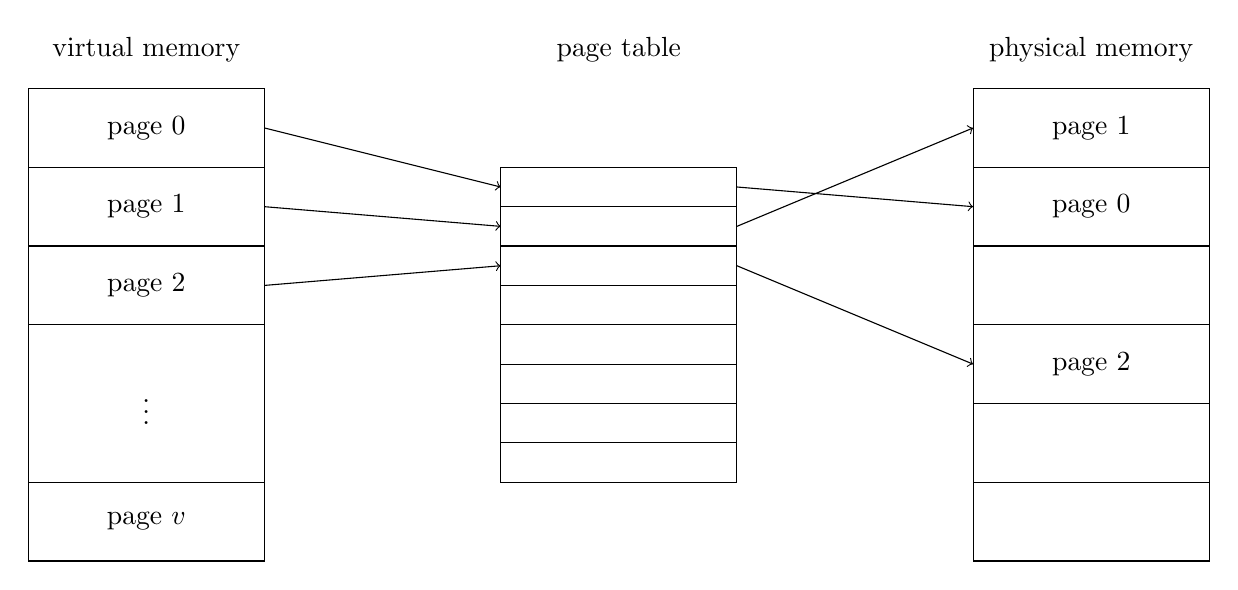
\begin{tikzpicture}[x=3cm]
                        \node at (0.5, 0.5) {virtual memory};
                        \node at (2.5, 0.5) {page table};
                        \node at (4.5, 0.5) {physical memory};
                        \node at (0.5, -0.5) {page 0};
                        \node at (0.5, -1.5) {page 1};
                        \node at (0.5, -2.5) {page 2};
                        \node at (4.5, -1.5) {page 0};
                        \node at (4.5, -0.5) {page 1};
                        \node at (4.5, -3.5) {page 2};
                        \node at (0.5, -4) {$\vdots$};
                        \node at (0.5, -5.5) {page $v$};
                        \draw
                        (1, -0.5) edge[->] (2, -1.25)
                        (3, -1.25) edge[->] (4, -1.5)
                        (1, -1.5) edge[->] (2, -1.75)
                        (3, -1.75) edge[->] (4, -0.5)
                        (1, -2.5) edge[->] (2, -2.25)
                        (3, -2.25) edge[->] (4, -3.5);
                        \draw
                        (0, 0) -- (1, 0) -- (1, -6) -- (0, -6) -- cycle
                        (0, -1) -- (1, -1)
                        (0, -2) -- (1, -2)
                        (0, -3) -- (1, -3)
                        (0, -5) -- (1, -5);
                        \draw
                        (2, -1) -- (3, -1) -- (3, -5) -- (2, -5) -- cycle
                        (2, -1.5) -- (3, -1.5)
                        (2, -2) -- (3, -2)
                        (2, -2.5) -- (3, -2.5)
                        (2, -3) -- (3, -3)
                        (2, -3.5) -- (3, -3.5)
                        (2, -4) -- (3, -4)
                        (2, -4.5) -- (3, -4.5);
                        \draw
                        (4, 0) -- (5, 0) -- (5, -6) -- (4, -6) -- cycle
                        (4, -1) -- (5, -1)
                        (4, -2) -- (5, -2)
                        (4, -3) -- (5, -3)
                        (4, -4) -- (5, -4)
                        (4, -5) -- (5, -5);
                    \end{tikzpicture}
                \end{center}
            \subsubsection*{Tutorial Questions}
                \begin{enumerate}[1.]
                    \itemsep0em
                    \item What is the advantage of a paged virtual memory system with;
                        \begin{enumerate}[(a)]
                            \itemsep0em
                            \item a small page size \hfill less unused memory (less fragmentation)
                            \item a large page size \hfill less entries in page table (less overhead, and faster access)
                        \end{enumerate}
                    \item Describe how a context switch affects the virtual memory system.
                        \medskip

                        The page table needs to be changed, as the page table is process specific.
                        This updates the base register in the MMU.
                        It also needs to clear cached address translations.
                \end{enumerate}
            \subsubsection*{Address Translation}
                Memory is byte addressable, and therefore memory addresses should refer to a specific byte in memory.
                For a logical address space $2^m$, and a page size of $2^n$, the address generated by the CPU should be divided into the page number $p$ (which is used as the index into the page table, which contains the base addresses of pages in physical memory), and the page offset $d$, which is which byte in the page we want to access.
                The page offset is the least significant (last) $n$ bits, and the page number is the remaining $m - n$ bits.
                Due to the size of the frame being the same as the size of the page, the offset does not need to change;
                \begin{center}
                    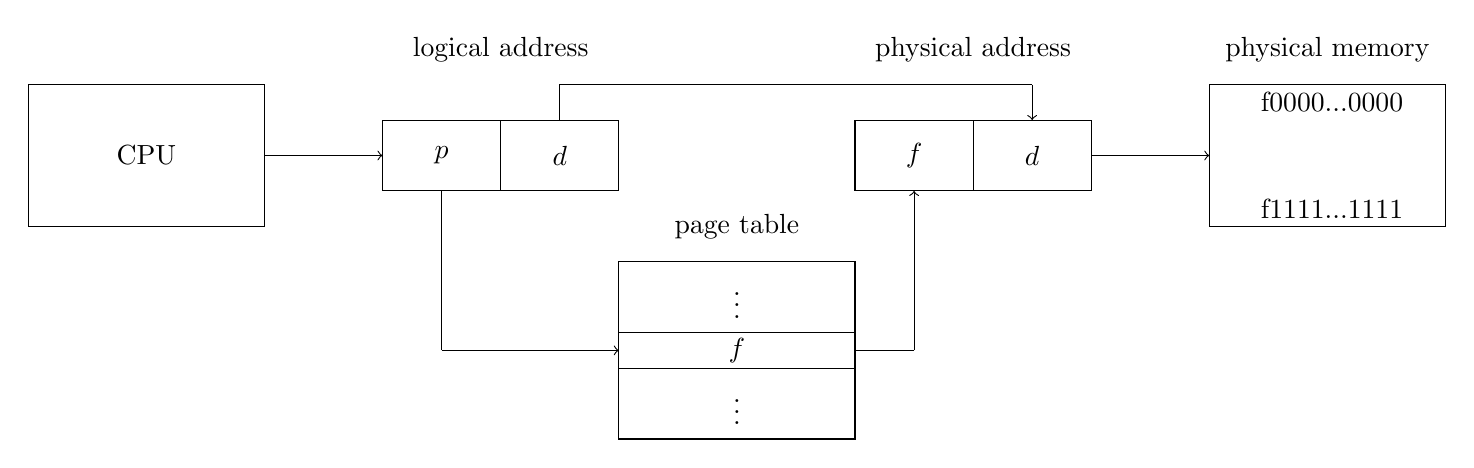
\begin{tikzpicture}[x=1.5cm, y=0.9cm]
                        \node at (4, 0.5) {logical address};
                        \node at (8, 0.5) {physical address};
                        \node at (11, 0.5) {physical memory};
                        \node at (6, -2) {page table};
                        \node at (1, -1) {CPU};
                        \node at (3.5, -1) {$p$};
                        \node at (4.5, -1) {$d$};
                        \node at (7.5, -1) {$f$};
                        \node at (8.5, -1) {$d$};
                        \node at (6, -3) {$\vdots$};
                        \node at (6, -3.75) {$f$};
                        \node at (6, -4.5) {$\vdots$};
                        \draw
                        (0, 0) -- (2, 0) -- (2, -2) -- (0, -2) -- cycle
                        (3, -0.5) -- (5, -0.5) -- (5, -1.5) -- (3, -1.5) -- cycle
                        (4, -1.5) -- (4, -0.5)
                        (7, -0.5) -- (9, -0.5) -- (9, -1.5) -- (7, -1.5) -- cycle
                        (8, -1.5) -- (8, -0.5)
                        (5, -2.5) -- (7, -2.5) -- (7, -5) -- (5, -5) -- cycle
                        (5, -3.5) -- (7, -3.5)
                        (5, -4) -- (7, -4);

                        \draw (2, -1) edge[->] (3, -1);
                        \draw (9, -1) edge[->] (10, -1);
                        \draw (3.5, -1.5) -- (3.5, -3.75) edge[->] (5, -3.75);
                        \draw (7, -3.75) -- (7.5, -3.75) edge[->] (7.5, -1.5);
                        \draw (4.5, -0.5) -- (4.5, 0) -- (8.5, 0) edge[->] (8.5, -0.5);

                        \draw
                        (10, 0) -- (12, 0) -- (12, -2) -- (10, -2) -- cycle;

                        \node at (11, -0.25) {~f0000...0000~};
                        \node at (11, -1.75) {~f1111...1111~};
                    \end{tikzpicture}
                \end{center}
                Note that it's also important to maintain a list of free frames, which are then taken to update the page table for a new process.
            \subsubsection*{Memory Protection}
                In the page table, we attach a valid-invalid bit to each entry;
                \begin{itemize}
                    \itemsep0em
                    \item \textbf{valid} indicates a legal page (has been allocated, and is mapped to physical memory)
                    \item \textbf{invalid} indicates the page is missing, either from the page not being in the process' virtual address space (page fault), or it exists but needs to be loaded from disk (demand paging) - kernel deals with this page fault
                \end{itemize}
                As each page table entry is just the frame address (as the offset is discarded), this can be stored in that part as simple book-keeping data.
            \subsubsection*{Tutorial / Exam Question}
                An embedded system uses a 16-bit big-endian architecture.
                It supports virtual memory management with a one-level page table.
                It has a page size of 1 KByte.
                The least significant bit of each page table entry represent a valid bit; the second least significant bit is the modified (dirty) but.
                The following are the current entries in the page table;
                \begin{center}
                    ~0x2C00~ \\
                    ~0x2403~ \\
                    ~0xCC01~ \\
                    ~0x0000~ \\
                    ~0x7C01~
                \end{center}
                Translate the following virtual memory addresses to physical memory addresses using the page table given above (if possible);
                \begin{enumerate}[(i)]
                    \itemsep0em
                    \item ~0xB85~ \hfill ~0b0000101110000101~
                        \medskip

                        Looking at the first 6 bits, it's in page table entry 2, hence it is address ~0b1100111110000101~, which is ~0xCF85~
                    \item ~0x1420~ \hfill ~0b0001010000100000~
                        \medskip

                        Looking at the first 6 bits, it's in page table entry 5, which doesn't exist, hence it page faults (beyond end)
                    \item ~0x1000~ \hfill ~0b0001000000000000~
                        \medskip

                        Looking at the first 6 bits, it's in page table entry 4, hence it is address ~0b0111110000000000~, which is ~0x7C00~
                    \item ~0xC9A~ \hfill ~0b0000110010011010~
                        \medskip

                        Looking at the first 6 bits, it's in page table entry 3, which is marked as invalid.
                \end{enumerate}
                The page size is $2^10$ bytes, hence the least significant 10 bits are used for the offset.
        \subsection*{13th November 2019}
            This starts with the exam question shown last lecture.
            Note that all of the translations we just manually performed must be done at every memory access.
            This overhead is outweighed by the flexibility of virtual memory.
            \subsubsection*{Page Table Implementation}
                We need to look at the representation of the page table, as it can grow very large, as well as handle the performance impacts caused by the overhead of using page tables.
                The page table is kept in main memory, and the page table base register (PTBR) points to the base of the page table, and the page table length register (PTLR) indicates the size.
                This needs to be changed when the processor switches processes.
                \medskip

                As previously mentioned, we now need to perform two memory accesses per data access; one for the page table, and one for the actual data.
                Most modern CPUs cache frequently translated memory addresses - this is done in hardware (in order to achieve very high performance), and uses this cache as associative memory (supporting parallel search).
                This is referred to as the translation look-aside buffer (TLB).
                The cache can be thought of as a table which holds the page number and frame number - before accessing the page table on memory, it checks if the page is in associative register, and if it is; it can obtain the frame number, otherwise the frame number has to be obtained from the table in memory.
                Some also store address-space identifiers (ASIDs) in entries, which uniquely identify each process to provide address-space protection.
                This cache needs to be flushed on a context switch (this is another overhead of context switches; initially the memory access will be slower) - the kernel can be mapped into every virtual address space to prevent this issue.
                \medskip

                We can calculate the effective access time as follows;
                \begin{align*}
                    \text{associative lookup} & = \epsilon \\
                    \text{assume memory cycle time} & = 1 & \mu\text{sec} \\
                    \text{hit ratio} & = \alpha & \text{page found in associative registers} \\
                    \text{EAT} & = (\epsilon + 1)\alpha + (\epsilon + 2)(1 - \alpha) \\
                    & = 2 + \epsilon - \alpha
                \end{align*}
                If our hit ratio is close to 1, then we have a very low overhead for paging.
            \subsubsection*{Page Table Size}
                As we are thinking of the page table as an array, each storing an address (4 bytes on 32-bit, 8 bytes on 64-bit), the sizes can be an issue.
                For example, on a 32-bit machine with 4KB pages, the page table will be at least 4MB, which is manageable.
                However, on a 64-bit machine, with 4KB pages, the page table will need $2^{52}$ entries.
                At 8 bytes per entry, that will be over 30 million GB.
                While we will have a very large address space, we are unlikely to actually need it all, and many entries in the page table will be unmapped.
                Some approaches are as follows;
                \begin{itemize}
                    \itemsep0em
                    \item hierarchical page table
                        \medskip

                        In a two-level page table, the outer page table will point to an inner page table (which handles all addresses falling within that range), instead of a frame.
                        The inner page table will only exist if there is at least one address in that range, meaning that we don't need to allocate a page table for the entire address space.
                        From the inner page table, we can get the actual frame.
                        \medskip

                        In this scenario, we're still assuming a 32-bit machine with a 1K page size.
                        The page offset therefore has to consist of 10 bits, and and a page number of 22 bits.
                        Since we've split the page tables, we also need to split the page number into a 12-bit page number ($p_1$), and a 10-bit page offset ($p_2$).
                        $p_1$ is the index into the outer page table, and $p_2$ is the displacement within the page that the outer page table is pointing too.
                        This can be expanded further with larger address spaces.
                        \begin{center}
                            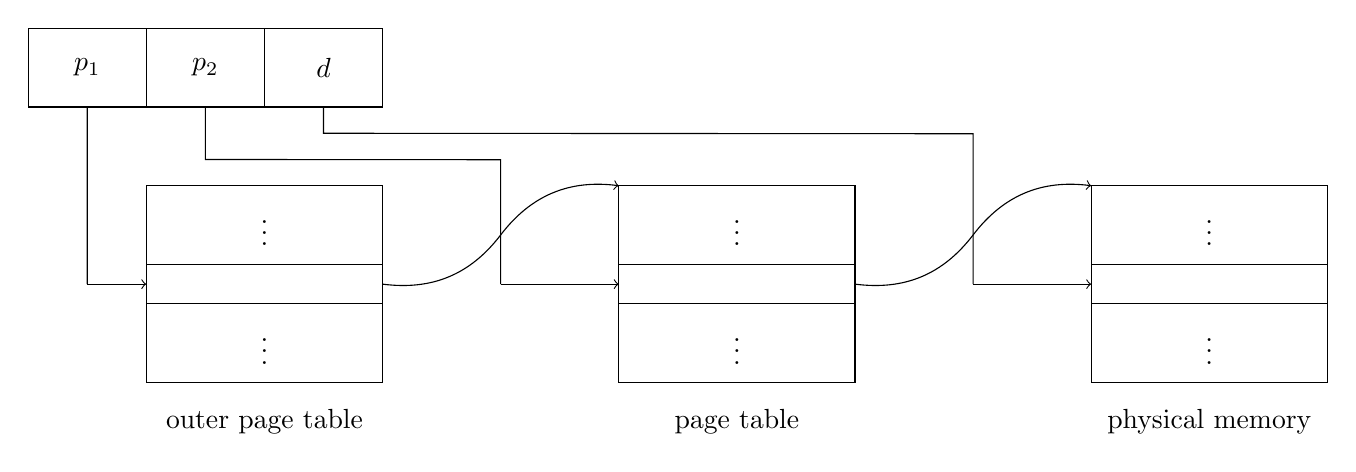
\begin{tikzpicture}[x=1.5cm]
                                \node at (6, -3) {outer page table};
                                \node at (10, -3) {page table};
                                \node at (14, -3) {physical memory};
                                \node at (4.5, 1.5) {$p_1$};
                                \node at (5.5, 1.5) {$p_2$};
                                \node at (6.5, 1.5) {$d$};
                                \draw
                                (4, 2) -- (7, 2) -- (7, 1) -- (4, 1) -- cycle
                                (5, 2) -- (5, 1)
                                (6, 2) -- (6, 1);

                                \node at (6, -0.5) {$\vdots$};
                                \node at (6, -2) {$\vdots$};
                                \draw
                                (5, 0) -- (7, 0) -- (7, -2.5) -- (5, -2.5) -- cycle
                                (5, -1) -- (7, -1)
                                (5, -1.5) -- (7, -1.5);

                                \node at (10, -0.5) {$\vdots$};
                                \node at (10, -2) {$\vdots$};
                                \draw
                                (9, 0) -- (11, 0) -- (11, -2.5) -- (9, -2.5) -- cycle
                                (9, -1) -- (11, -1)
                                (9, -1.5) -- (11, -1.5);

                                \node at (14, -0.5) {$\vdots$};
                                \node at (14, -2) {$\vdots$};
                                \draw
                                (13, 0) -- (15, 0) -- (15, -2.5) -- (13, -2.5) -- cycle
                                (13, -1) -- (15, -1)
                                (13, -1.5) -- (15, -1.5);

                                \draw
                                (7, -1.25) edge[bend right=30] (8, -0.625)
                                (8, -0.625) edge[->, bend left=30] (9, 0)
                                (11, -1.25) edge[bend right=30] (12, -0.625)
                                (12, -0.625) edge[->, bend left=30] (13, 0);

                                \draw
                                (4.5, 1) -- (4.5, -1.25) edge[->] (5, -1.25)
                                (5.5, 1) -- (5.5, 0.333) -- (8, 0.33) -- (8, -1.25) edge[->] (9, -1.25)
                                (6.5, 1) -- (6.5, 0.666) -- (12, 0.66) -- (12, -1.25) edge[->] (13, -1.25);
                            \end{tikzpicture}
                        \end{center}
                        However, this makes memory access even slower, since we need to do more accesses.
                    \item hashed page table
                        \medskip

                        Ideally we'd want a structure for a page table that grows with the number of frames, which is a data structure that is linear with the physical memory.
                        Here, the page table contains a chain of elements hashing to the same location, and we can search for a match of the virtual page number in the chain.
                        This gives us the exact corresponding physical frame if a match is found.
                        However, this is more difficult to implement as it has to be done in hardware, including the hashing function.
                    \item inverted page table
                        \medskip

                        Index the page table by the frame address.
                        Each entry then contains a page address and the process identifier.
                        This way the structure grows with the frames, however this increases the time as each lookup now requires a linear search through the table.
                \end{itemize}
            \subsubsection*{Tutorial Question}
                Assuming that time for a memory access is 100ns, and for TLB access 20ns.
                Calculate the access times for a four-level paging system assuming a TLB hit ratio of
                \begin{enumerate}[(a)]
                    \itemsep0em
                    \item 80\%
                        \medskip

                        The time for translation is $0.8 \cdot (100 + 20) + 0.2 \cdot (500 + 20)$, which is 200ns - thus 100\% slower than unpaged memory access (with one level, it is 140ns, thus 40\%).
                    \item 98\%
                        \medskip

                        The time for translation is $0.98 \cdot (100 + 20) + 0.02 \cdot (500 + 20)$, which is 128ns - thus 28\% slower than unpaged memory access (with one level, it is 122ns, thus 22\%).
                \end{enumerate}
        \subsection*{14th November 2019}
            \subsubsection*{Tutorial Question}
                \begin{enumerate}[1.]
                    \itemsep0em
                    \item
                        A pure paging system uses a three level page table.
                        Virtual addresses are decomposed into four fields $(a, b, c, d)$ with $d$ being the offset.
                        In terms of these constants, what is the maximum number of pages in a virtual address space?
                        \medskip

                        $2^{a + b + c}$, since we have $2{a + b + c + d}$ total addresses, and $2^d$ on each page.
                \end{enumerate}
            \subsubsection*{Shared Memory}
                The idea is that there is memory accessible from two (or more) processes.
                This creates a mechanism for two processes to communicate.
                When process 1 attempts to access the shared page, the page table entry will point it to the same frame that process 2 points to, and vice versa.
                \begin{center}
                    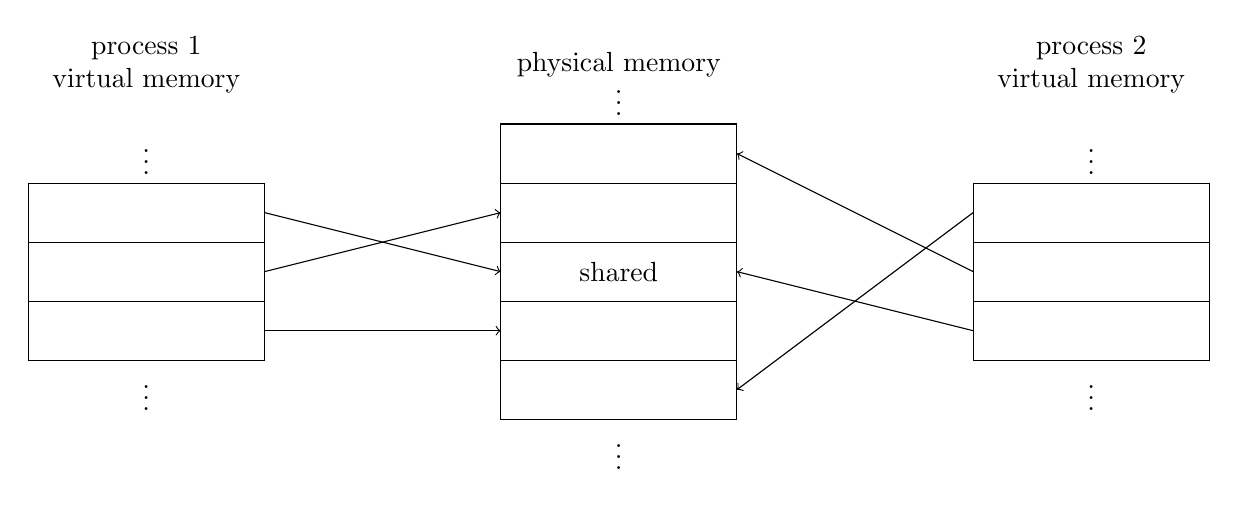
\begin{tikzpicture}[x=1.5cm, y=0.75cm]
                        \node at (1, 2) {\shortstack{process 1\\virtual memory}};
                        \node at (5, 2) {physical memory};
                        \node at (9, 2) {\shortstack{process 2\\virtual memory}};
                        \node at (1, 0.5) {$\vdots$};
                        \node at (1, -3.5) {$\vdots$};
                        \node at (5, 1.5) {$\vdots$};
                        \node at (5, -4.5) {$\vdots$};
                        \node at (9, 0.5) {$\vdots$};
                        \node at (9, -3.5) {$\vdots$};
                        \node at (5, -1.5) {shared};
                        \draw
                        (0, 0) -- (2, 0) -- (2, -3) -- (0, -3) -- cycle
                        (0, -1) -- (2, -1)
                        (0, -2) -- (2, -2)
                        (4, 1) -- (6, 1) -- (6, -4) -- (4, -4) -- cycle
                        (4, 0) -- (6, 0)
                        (4, -1) -- (6, -1)
                        (4, -2) -- (6, -2)
                        (4, -3) -- (6, -3)
                        (8, 0) -- (10, 0) -- (10, -3) -- (8, -3) -- cycle
                        (8, -1) -- (10, -1)
                        (8, -2) -- (10, -2);
                        \draw
                        (2, -0.5) edge[->] (4, -1.5)
                        (2, -1.5) edge[->] (4, -0.5)
                        (2, -2.5) edge[->] (4, -2.5)
                        (8, -0.5) edge[->] (6, -3.5)
                        (8, -1.5) edge[->] (6, 0.5)
                        (8, -2.5) edge[->] (6, -1.5);
                    \end{tikzpicture}
                \end{center}
                After this is established, it appears as memory both processes can access, therefore there is no need for kernel involvement (hence no need for the context switching overhead).
                To establish this, there are the following system calls;
                \begin{center}
                    \begin{tabular}{ll}
                        call & explanation \\
                        \hline
                        ~shmget~ & allocates a shared memory segment \\
                        ~shmat~ & attaches a shared memory segment to the address space of a process \\
                        ~shmctl~ & change properties associated with a shared memory segment \\
                        ~shmdt~ & detaches a shared memory segment from a process
                    \end{tabular}
                \end{center}
                It would be better for two processes to communicate via pipes due to the flexibility of bi-directional communication, however it's not better for uni-directional communication as there is no synchronisation provided by the kernel (compared to pipes).
                Because the kernel provides no abstractions for this, synchronisation between two processes using the same shared memory will have to be done in a similar way to two threads concurrently executing on the same memory (locking, etc).
                \medskip

                As this can also be mapped to a file (and not just a location on main memory), this can be used for dynamic linking of libraries - thus allowing for libraries to be shared.
            \subsubsection*{Linux Virtual Memory Layout (32-bit)}
                \begin{center}
                    \begin{tikzpicture}
                        \node at (0, 0.5) {0};
                        \node at (10, 0.5) {896MB};
                        \node at (0, -7.5) {0};
                        \node at (6, -7.5) {3GB};
                        \node at (17, -7.5) {4GB};
                        \node[rotate=90] at (-0.5, -1) {main memory};
                        \node[rotate=90] at (-0.5, -6) {virtual memory};
                        \node at (1, -1) {DMA};
                        \node at (6.5, -1) {normal memory};
                        \node at (13, -1) {high memory};
                        \node at (3, -6) {user process};
                        \draw
                        (0, 0) -- (12, 0)
                        (12, 0) edge[dashed] (14, 0)
                        (14, 0) -- (16, 0)
                        (0, -2) -- (12, -2)
                        (12, -2) edge[dashed] (14, -2)
                        (14, -2) -- (16, -2)
                        (0, -2) -- (0, 0)
                        (2, -2) -- (2, 0)
                        (3, -2) -- (3, 0)
                        (16, -2) -- (16, 0)
                        (10, -2) -- (10, 0);
                        \draw
                        (0, -5) -- (2, -5)
                        (2, -5) edge[dashed] (4, -5)
                        (4, -5) -- (17, -5)
                        (0, -7) -- (2, -7)
                        (2, -7) edge[dashed] (4, -7)
                        (4, -7) -- (17, -7)
                        (0, -7) -- (0, -5)
                        (6, -7) -- (6, -5)
                        (8, -7) -- (8, -5)
                        (9, -7) -- (9, -5)
                        (16, -7) -- (16, -5)
                        (17, -7) -- (17, -5);
                        \draw[dashed]
                        (0, -2) edge[<->] (6, -5)
                        (2, -2) edge[<->] (8, -5)
                        (3, -2) edge[<->] (9, -5)
                        (10, -2) edge[<->] (16, -5);
                    \end{tikzpicture}
                \end{center}
                Note that the $n^\text{th}$ page of the kernel address space (3GB - 4GB in virtual memory) maps to the $n^\text{th}$ page frame of main memory.
                For legacy reasons, we have the interrupt vectors stored at low addresses.
                DMA is used for direct memory access from I/O devices, such as network cards, to allow them to write to memory, bypassing the CPU.
                The kernel address space is mapped into virtual memory as well, meaning that when a system call is performed, the page tables don't have to be switched thus removing that overhead.
                The additional space at the end of virtual memory is used for on-demand mapping, which is done when the kernel wants to access physical memory beyond the 896MB boundary, by creating inserting a mapping into the page table (this isn't needed for 64-bit architectures, as we can map the entirety of main memory).
                A process attempting to access beyond the 3GB boundary will result in a page fault, as it is essentially attempting to access privileged kernel memory.
                Another benefit of having a larger address space is that the operating system can randomise the locations of data structures and libraries, making it more difficult for an attacker to locate a vulnerable library.
                \medskip

                On IA-32, the page size is usually 4KB, with a 4GB virtual address space, whereas on x86-64, there are larger page sizes (such as 4MB), and up to a four-level page table.
                The implementation of the two-level page table in x86 is as previously discussed (the outer page table is referred to as the \textbf{page global directory}).
                As the offset bits are unused, it will be used to store the metadata, such as dirty, read / write, etc.
            \subsubsection*{Meltdown (Not Examinable)}
                \begin{lstlisting}
                    ...
                    if (v == 0) {
                      w = kernel_mem[addr];
                      x = w & 0x01;
                      y = x * 4096;
                      z = user_mem[u];
                    }
                \end{lstlisting}
                By speculative execution, it executes the code in the branch.
                It will not page fault straight away, as that branch may not be reached - however the instructions will be executed.
                Looking at the last bit of the data stored in the kernel address will result in an access to the user memory at either 0 or 4096, bringing it into cache.
                The attacker can then check how long it takes to access these (the one with the faster access has been brought into cache).
                To fix this, Linux moved the kernel address space into its own virtual address space, thus requiring a context switch.
                Due to the additional complexity, the processor cannot speculate across this.
            \subsubsection*{Demand Paging}
                The idea behind this is to think of pages for programs which aren't currently running as swapped out.
                We are then only loading pages on demand; consider the example of running a large binary - we don't need to load the entire binary into memory before execution, as we only need the instructions for the main entry point.
                When we encounter a page fault, it may still be caused by an actual invalid reference, but also may be caused by the page not being in memory (thus requiring the OS to load it in).
                \medskip

                To indicate whether something is in memory, we use the valid-invalid bit, with everything initially set to 0.
                If it is 1 during address translation, we simply bring it in as before, but if it is 0, we let the OS trap the page fault.
                This is then checked against another table, if it is still invalid, we abort, otherwise we handle the request.
                This is done by obtaining an empty frame, swapping the page into the frame, setting the table's valid bit to 1, and restarting the instruction that caused the fault.
                \medskip

                We can reason about this in a similar way, with a page fault rate $0 \leq p \leq 1$, where if $p = 0$, we have no page faults.
                The effective access time is $(1 - p) \cdot \text{memory access} + p \cdot (\text{page fault overhead} + \text{page swap out?} + \text{page swap in} + \text{restart overhead})$.
                If a free frame is not available, a page may have to be swapped out.
                Overall, we have a much higher overhead; with insufficient memory, this leads to thrashing due to the I/O overhead the OS must perform for this swapping.
                \medskip

                Virtual memory allows us to do the following;
                \begin{itemize}
                    \itemsep0em
                    \item \textbf{copy-on-write}
                        \medskip

                        This is useful in ~fork~, as we share many of the pages (thus it would be very wasteful to copy it all).
                        When either process modifies a shared page, only then do we copy them.
                    \item \textbf{memory-mapped files}
                        \medskip

                        When we memory map a file, associating it with pages in the virtual address space, we bring them in on the first access with demand paging.
                        This is a very efficient way of performing I/O on large files, as we do not need the overhead of system calls.
                \end{itemize}
            \subsubsection*{Page Replacement}
                When we are out of free frames on main memory, we need to find an unused page that we can swap out.
                Our policy must minimise the number of page faults (ideally replacing one that will not be used), ensure that we do not over-allocate memory, and ensuring that only modified (dirty) pages to write to disk (we shouldn't write an unmodified page to the disk).
                The dirty bit is set by hardware on a write.
                A basic replacement algorithm is as follows;
                \begin{itemize}
                    \itemsep0em
                    \item find location of desired page on disk
                    \item find a free frame, if one is not found, we select a victim frame
                    \item read the desired page into the frame
                    \item update page and frame tables
                    \item restart the process
                \end{itemize}
                Some eviction algorithms are as follows;
                \begin{itemize}
                    \itemsep0em
                    \item \textbf{first-in-first-out (FIFO)}
                        \medskip

                        This simply evicts the oldest page - this may however replace a heavily used page.
                        This suffers from Belady's anomaly, where we have can have more page faults with more physical frames.
                    \item \textbf{optimal algorithm}
                        \medskip

                        The theoretical optimal is to evict the page that won't be used for the longest time.
                        This obviously cannot be done (perfectly or easily) in practice, but can be used to judge how well another page replacement strategy performs.
                \end{itemize}
        \subsection*{27th November 2019}
            \subsubsection*{Page Replacement}
                This continues with page eviction algorithms.
                \begin{itemize}
                    \itemsep0em
                    \item \textbf{least recently used (LRU)}
                        \medskip

                        The idea for this algorithm is to evict the least recently used (since it's possible that the program no longer requires this page), via the use of a counter (per page entry).
                        On a reference, the clock is copied into the counter, and when a page needs to be replace, we choose to evict the one with the lowest counter.
                        However, this is expensive as we need to copy the entire counter, and we use single register approximations.
                    \item \textbf{reference bit}
                        \medskip

                        This is an approximation of LRU, but does not provide proper order.
                        We associate a reference bit with each page, initially set to 0.
                        When it is referenced, it is set to 1 (can be set by hardware), and on a replacement it attempts to find a page with the bit set to 0.
                        Periodically, all the reference bits are reset to 0.
                    \item \textbf{second chance / clock}
                        \medskip

                        This uses the idea of a reference bit, as well as an order of when pages are brought into memory.
                        When a page is brought into memory, it is stored in a linked list.
                        We have a pointer into the linked list (clock hand) which points at the oldest page.
                        If this page has a reference bit of 0, then we evict it, however if it is 1, we set it to 0, and move to the second oldest page.
                        This continues until we find a page that can be evicted.
                        The idea behind this is that while a page may be old, if it was recently accessed, it may still be in use, and we wouldn't want to evict that.
                    \item \textbf{least frequently used (LFU)}
                        \medskip

                        The previous algorithms do not take into account the frequency of accesses, just that it was or wasn't.
                        For this algorithms, we maintain a count of the number of references.
                        Here we replace the page with the smallest count - however this may replace a page that was recently brought in.
                        Additionally, if there was a heavily used page that is no longer needed, it may not be evicted - we need to reset counters or age the counters.
                    \item \textbf{most frequently used (MFU)}
                        \medskip

                        Replace pages with a large count - if we haven't used it recently, then it's likely it is no longer needed.
                        While this may seem counterintuitive, memory accesses tend to fall within working sets; after a data structure is no longer used, it will no longer experience more references.
                \end{itemize}
            \subsubsection*{Locality of Reference}
                A property of many programs is that it tends to favour a subset of pages, which it accesses most frequently.
                There is locality of space as well as time - for example, iterating over a data structure gives spatial locality, and doing this repeatedly gives us temporal locality.
                This also gives better performance due to the caching in the TLB, preventing the walk through the page tables.
                \medskip

                We define the working set of pages as $W(t, w)$ - the set of pages referenced by a process during the time interval $t - w$ to $t$.
                The working set can change over time for a given process.
                This can be used with the WS clock algorithm, by tracking the "time of last use".
                At each page fault, we do the following check on the page we're pointing at;
                \begin{itemize}
                    \itemsep0em
                    \item if the referenced bit is set to 1, reset it to 0, and move to the next page
                    \item if the referenced bit is not set, we calculate its age
                        \begin{itemize}
                            \itemsep0em
                            \item if the age is less than the working set age, continue (as the page is in the WS)
                            \item if the age is older than the working set age, we replace it (writing back to disk if required)
                        \end{itemize}
                \end{itemize}
                We however need to model the size of the working set.
                This can be done by observing the page fault frequency - if we estimate incorrectly (too low), we will encounter many page faults, thus having a low interval between page faults.
                If $w$ is too high, thus we are assuming the working set is larger than it is, we will have diminishing returns (the page fault frequency doesn't change, as the entire working set is now in pages).
                We can tune this dynamically.
                \medskip

                A local page replacement strategy is when each process gets a fixed allocation of physical memory, and we need to pick up the changes in the working set size.
                On the other hand, a global strategy dynamically shares memory between runnable processes, and considers page fault frequency to tune allocation (gives more to a process by taking from another).
                Linux uses a global page replacement strategy, whereas Windows uses local.
            \subsubsection*{Linux Page Replacement}
                Linux uses a variation of the clock algorithm (to approximate LRU).
                The memory manager uses two linked list (as well as reference bits) - the active list containing active pages, with the most recently used pages near the head of the active list, as well as an inactive list, which has the least-recently used pages near the tail.
                Unused pages from the active list are moved to the head of the inactive list.
                It only replaces pages in the inactive list.
                \medskip

                From a practical point of view, we cannot simply perform this eviction on a fault, as we don't tend to have the granularity of allocating memory in just pages.
                For example, if the memory was full, and we performed a ~malloc~ for a large amount of memory, we don't want to do many evictions as that would be slow.
                Instead, this is done asynchronously by the following (when the processor is idle);
                \begin{itemize}
                    \itemsep0em
                    \item ~kswapd~ (swap daemon)
                        \subitem reclaims pages in the inactive list when memory is low to a dedicated swap partition or file, and handles locked and shared pages
                    \item ~pdflush~ (kernel thread)
                        \subitem periodically flushes dirty pages to disk (allows for easier eviction) - done when there is low I/O load
                \end{itemize}
            \subsubsection*{Tutorial Question}
                Suppose that pages in a virtual address space are referenced in the following order;
                \begin{center}
                    ~1 2 1 3 2 1 4 3 1 1 2 4 1 5 6 2 1~
                \end{center}
                There are 3 empty frames available.
                Assume that paging decisions are made on demand, i.e. when page faults occur.
                Show the contents of the frames after each memory reference (and how many page faults occur in each case), assuming
                \begin{enumerate}[(a)]
                    \itemsep0em
                    \item the LRU replacement policy \hfill 11 faults
                        \begin{center}
                            \begin{tabular}{l|ccccccccccccccccc}
                                \multirow{2}{*}{frame} & \multicolumn{17}{c}{reference} \\
                                & 1 & 2 & 1 & 3 & 2 & 1 & 4 & 3 & 1 & 1 & 2 & 4 & 1 & 5 & 6 & 2 &  1 \\
                                \hline
                                0 & 1 & 1 & 1 & 1 & 1 & 1 & 1 & 1 & 1 & 1 & 1 & 1 & 1 & 1 & 1 & 2 & 2 \\
                                1 &   & 2 & 2 & 2 & 2 & 2 & 2 & 3 & 3 & 3 & 3 & 4 & 4 & 4 & 6 & 6 & 6 \\
                                2 &   &   &   & 3 & 3 & 3 & 4 & 4 & 4 & 4 & 2 & 2 & 2 & 5 & 5 & 5 & 1 \\
                                fault & $\times$ & $\times$ & & $\times$ & & & $\times$ & $\times$ & & & $\times$ & $\times$ & & $\times$ & $\times$ & $\times$ & $\times$
                            \end{tabular}
                        \end{center}
                    \item the clock policy \hfill 9 faults
                        \begin{center}
                            \begin{tabular}{l|ccccccccccccccccc}
                                \multirow{2}{*}{frame} & \multicolumn{17}{c}{reference} \\
                                & 1 & 2 & 1 & 3 & 2 & 1 & 4 & 3 & 1 & 1 & 2 & 4 & 1 & 5 & 6 & 2 &  1 \\
                                \hline
                                0 & 1 & 1 & 1 & 1 & 1 & 1 & 4 & 4 & 4 & 4 & 4 & 4 & 4 & 5 & 5 & 5 & 5 \\
                                1 &   & 2 & 2 & 2 & 2 & 2 & 2 & 2 & 1 & 1 & 1 & 1 & 1 & 1 & 6 & 6 & 6 \\
                                2 &   &   &   & 3 & 3 & 3 & 3 & 3 & 3 & 3 & 2 & 2 & 2 & 2 & 2 & 2 & 1 \\
                                fault & $\times$ & $\times$ & & $\times$ & $\times$ & & $\times$ & & $\times$ & & $\times$ & & & $\times$ & $\times$ & &
                            \end{tabular}
                        \end{center}
                \end{enumerate}
        \subsection*{28th November 2019}
            This starts with the tutorial question given at the end of the last lecture.
            \subsubsection*{Device Management}
                The goals for an OS regarding device management are the following;
                \begin{itemize}
                    \itemsep0em
                    \item fair access (processes competing for resources such as disk, network card etc.)
                    \item exploit parallelism (such as SSD access)
                    \item hide complexity of I/O devices
                \end{itemize}
                We also want device independence from both the type (terminal, disk, DVD etc.) and the instance (which disk it's actually referring to).
                We want to have the following properties for each device class (what they can achieve);
                \begin{itemize}
                    \itemsep0em
                    \item unit of data transfer
                        \begin{itemize}
                            \itemsep0em
                            \item character \hfill input devices one character at a time
                            \item block \hfill fixed sized blocks
                                \subitem makes more sense to read / write a large amount of data than many individual requests
                        \end{itemize}
                        \begin{center}
                            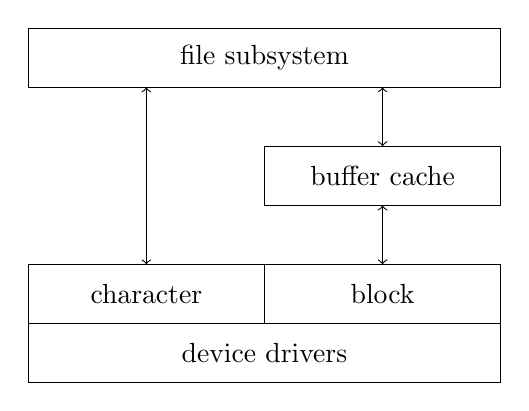
\begin{tikzpicture}[x=1.5cm, y=0.75cm]
                                \node at (2, -0.5) {file subsystem};
                                \node at (3, -2.5) {buffer cache};
                                \node at (1, -4.5) {character};
                                \node at (3, -4.5) {block};
                                \node at (2, -5.5) {device drivers};
                                \draw
                                (0, 0) -- (4, 0) -- (4, -1) -- (0, -1) -- cycle
                                (2, -2) -- (4, -2) -- (4, -3) -- (2, -3) -- cycle
                                (0, -4) -- (4, -4) -- (4, -6) -- (0, -6) -- cycle
                                (0, -5) -- (4, -5)
                                (2, -4) -- (2, -5);
                                \draw
                                (1, -1) edge[<->] (1, -4)
                                (3, -1) edge[<->] (3, -2)
                                (3, -3) edge[<->] (3, -4);
                            \end{tikzpicture}
                        \end{center}
                        When working with blocks, we can use a cache, whereas this isn't needed with characters.
                    \item supported operations \hfill read, write, seek, etc.
                    \item synchronous (block until response) or asynchronous (will raise interrupt on response)
                    \item shareable (such as disks) or single user (such as optical disk drives)
                        \medskip

                        A dedicated device needs a simple policy, such as failing to open a device if it is already opened, or queuing requests.
                        On the other hand, the OS can provide an abstracted file system which is then exposed to programs.
                    \item types of error conditions
                \end{itemize}
                In I/O layering, the rest of the OS needs to communicate with the drivers, which in turn communicate with the hardware controllers on the actual devices.
                At the top is user-level I/O software, followed by device-independent operating system software, then device drivers, interrupt handlers, and then the hardware.
                \begin{itemize}
                    \itemsep0em
                    \item \textbf{interrupt handler}
                        \medskip

                        This processes each interrupt received from an I/O device.
                        For block devices, this is signalled on the completion of a block (compared to an interrupt per character).
                        When a character is transferred, it needs to process the next character.
                        The interrupt handlers are needed as I/O devices behave in a fundamentally asynchronous fashion.
                    \item \textbf{device drivers}
                        \medskip

                        Specific to a type of device (implemented by the device manufacturer).
                        It can implement reading and writing to the device, access to the devices' registers, scheduling requests, and error handling (transparent to OS).
                        \medskip

                        Memory-mapped I/O allows a device to be addressed as a memory location.
                        \begin{itemize}
                            \itemsep0em
                            \item programmed I/O \hfill inefficient as we don't want to keep polling
                            \item interrupt-driven I/O \hfill hardware raises interrupt to be handled
                            \item DMA (direct memory access) \hfill bypassing CPU without interrupt
                                \subitem only raises one interrupt to the CPU once everything is done, reducing number of interrupts
                        \end{itemize}
                    \item \textbf{device independent OS layer}
                        \medskip

                        Attempts to standardise interface for a specific class of driver.
                        This provides device independence, such as naming devices (as we don't want processes to refer directly to physical device but our logical naming abstraction of it).
                        This is required since a component can be updated on a device, and the software would not be able to deal with it (if it were referring to a specific physical device).
                        \medskip

                        This layer also provides request validation - verifying that the operation we want to carry out is supported by the device.
                        It also gives us resource allocation for a device that can't be shared, as well as user access validation.
                        Buffering of blocks is also implemented in this layer, allowing it to be used across all devices.
                        \medskip

                        A way of allocating nonsharable devices is to use a process called spooling, instead of blocking each process until it is free.
                        An example of a spooled device is a printer, where the output is saved to a disk file first.
                        This is then printed out by a spooler daemon, which is the only process that has direct access to the printer.
                        This allows any process to send data to a printer, and have it eventually be printed.
                        \medskip

                        Buffered I/O means that all I/O requests to and from a device goes through this cache (transparent).
                        This gives better performance.
                        On the other hand, having unbuffered I/O goes directly from the user space to / from the device.
                        This has better latency, compared to the use of a buffer cache.
                        Another use of unbuffered I/O is for databases, as we want to have the guarantee of durability, and that we write to the disk straight away.
                    \item \textbf{user-level I/O interface}
                        \medskip

                        This is a higher abstraction we give to processes (device independent), and exposes both blocking and non-blocking APIs, from which the application can then choose what to use.
                        Unix gives an I/O API where everything is accessible as files - this allows the same API to be used for device I/O as for the file system.
                \end{itemize}
            \subsubsection*{Linux Implementation}
                Linux provides device drivers through the use of loadable kernel modules (LKM).
                Dynamically inject code into kernel - this contains object code which is loaded on demand, and is typically provided by the hardware vendor.
                However, as the code is being injected into the kernel, it requires binary compatibility, as modules written fro different kernel versions may not work together.
                Kmod is a kernel subsystem that manages modules on-demand, such as when a new device is plugged in.
                It also handles module dependencies, if there are any.
                Every LKM consists of at least two basic functions, and is loaded by ~insmod module.o~;
                \begin{lstlisting}
                    int init_module(void) {
                      // all initialisation code
                    }
                    void cleanup_module(void) {
                      // clean shutdown
                    }
                \end{lstlisting}
                Linux provides a common interface for I/O system calls.
                Devices are grouped into classes, where members perform similar functions (such as input devices).
                The individual devices are identified by major and minor identification numbers, where devices of the same major number are controlled by the same driver, and minor numbers allow the system to distinguish between devices of the same class.
                The devices can be listed by looking at the contents of ~/dev~ - which also shows the major and minor numbers.
                Therefore instead of writing to an actual file in ~/dev~, Linux will look up the device driver, which then sends the data to the device in question.
                \medskip

                While this abstraction is powerful, as we can have every operation go through the virtual file system (VFS) which distinguishes between a file system operation and a device operation, it cannot support all operations on devices.
                Additional functionality is done through the ~ioctl~ system call, which supports special tasks such as ejecting the CD-ROM tray, or retrieving status information from the printer.
                \medskip

                Devices are represented as follows in Linux;
                \begin{itemize}
                    \itemsep0em
                    \item character devices
                        \medskip

                        This transmits data as a stream of bytes, and is represented by a ~device\_struct~ which contains the driver name and a pointer to the driver's ~file\_operations~ structure.
                        All the registered drivers are referenced by the ~chrdevs~ vector.
                    \item block devices
                        \medskip

                        Due to the additional complexity, there is an entire block I/O subsystem.
                        The kernel also implements strategies to minimise the amount of time accessing block devices by caching data and clustering I/O operations.
                        \medskip

                        When data is requested from the block device, the kernel first attempts to search the block cache - if it is found the data is copied to the process' address space, otherwise it is added to the request queue.
                        Direct I/O is also supported, which bypasses the kernel cache.
                \end{itemize}
                The I/O classes are as follows;
                \begin{center}
                    \begin{tabular}{ll}
                        I/O class & types \\
                        \hline
                        character (unstructured) & files and devices \\
                        block (structured) & devices \\
                        pipes (message) & interprocess communication \\
                        socket (message) & network interface (bidirectional communication)
                    \end{tabular}
                \end{center}
                The API is as follows;
                \begin{itemize}
                    \itemsep0em
                    \item ~fd = create(filename, permission)~
                    \item ~fd = open(filename, mode)~ \hfill mode is 0, 1, or 2 for read, write, read and write
                    \item ~close(fd)~ \hfill release resources when done
                    \item ~bytesread = read(fd, buffer, numbytes)~ \hfill reads into ~buffer~, returns actual number read
                    \item ~byteswritten = write(fd, buffer, numbytes)~
                        \subitem writes into ~fd~ from ~buffer~, returns actual number written
                    \item ~fd = mknod(filename, permission, dev)~
                        \subitem creates a new special file (character or block device)
                \end{itemize}
                Each process has its own file descriptor table, with the first 3 (0, 1, 2) being ~stdin~, ~stdout~, and ~stderr~.
                These normally refer to the terminal that the process was started from.
            \subsubsection*{Blocking vs Non-blocking}
                With blocking I/O, the call returns when the operation completes, however during this time the processor is likely to context switch to something else, as this process is now waiting.
                This is easy to reason about, but can lead to multi-threaded code if work needs to be done in the background.
                On the other hand, non-blocking I/O does as much work as possible.
                To enable this for a file descriptor, the ~fcntl~ system call is used, and any future read / write to the file descriptor will give non-blocking semantics.
                Application-level polling now needs to be implemented.
                \medskip

                A more modern style of doing I/O is to do asynchronous I/O.
                This effectively provides a "callback", where a request is made to the kernel through a system call, which is then initiated.
                The application continues on (this is non-blocking), and once the kernel has a read response, it then signals the process that the operation is complete.
            \subsubsection*{Tutorial Question}
                In which of the four I/O software layers (user-level I/O software, device-independent OS software, device drivers and interrupt handlers) is each of the following done?
                \begin{enumerate}[(a)]
                    \itemsep0em
                    \item Computing the track, sector and head for a disk read \hfill device drivers
                    \item Maintaining a cache of recently used blocks \hfill device-independent OS software
                    \item Writing commands to the drive registers \hfill device drivers or interrupt handler
                    \item Checking to see if the user is permitted to use the device \hfill device-independent OS software
                    \item Converting binary integers to ASCII for printing \hfill user-level I/O software
                \end{enumerate}
        \subsection*{29th November 2019}
            \subsubsection*{Disk Management}
                Note that while the capacity of storage mediums grow exponentially, the same cannot be said for access speeds, due to physical limitations - for example HDDs must physically move components.
                The surface of a HDD is organised into tracks (rings), which are subdivided into sectors.
                Between each sector there is an inter-sector gap, and between tracks are inter-track gaps.
                Each platter can have 2 surfaces (one on each side) - and there is a read / write for each surface.
                For multiple platters, there are two read / write heads between each platter (other than the first and last).
                \medskip

                As all the arms move together, tracks which are on top of each other are referred to as a cylinder - and therefore can be read at the same time.
                Note that it's desirable to have the same size per sector.
                However, the inner tracks will physically have smaller sectors, therefore the outer tracks will have more sectors than the inner tracks.
                The zones are then exposed with virtual geometry, where it appears to have the same number of sectors per track.
                \medskip

                In the past, the disk was physically addressed with the cylinder, surface, and sector.
                Modern disks use logical sector addressing (or logical block addressing - LBA), where all sectors are numbered consecutively (thus the OS doesn't need to know about the physical geometry).
                \medskip

                It's also important to note that disk manufacturers use powers of 10, instead of powers of 2, for capacities - for the exam, either is fine as long as it is consistent.
                \medskip

                Before a disk is used, it needs to be formatted.
                At a low level, in addition to the actual data, each disk sector stores an ECC (error correction code) at the end, as well as a preamble, which can be used to indicate the start of a sector.
                In addition to this, there is a higher level formatting system.
            \subsubsection*{Tutorial Question}
                A disk controller with enough memory can perform read-ahead, reading blocks on the current track into its memory before the CPU asks for them.
                Should it also do write-behind, i.e. report back to the CPU that a block has been written once it is stored in the disk controller's memory?
                \medskip

                Not in general, as the OS should rely on a page remaining written even in the event of an immediate crash.
                Reporting this completion before writing violates this rule.
                A controller can only do write-behind if its local memory is battery backed for long enough that it can perform the write that was reported complete before the crash.
            \subsubsection*{Disk Delay}
                There are numerous points which contribute to the latency of using a disk (where $b$ is the number of bytes to be transferred, $N$ is the number of bytes per track, and $r$ is the rotation speed in revolutions per second);
                \begin{itemize}
                    \itemsep0em
                    \item seek time \hfill time it takes for the read / write head to move to the correct track ($t_\text{seek}$)
                    \item rotational delay / latency time \hfill time for the sector to be in the right place ($t_\text{latency} = \frac{1}{2r}$)
                    \item transfer time \hfill the actual time the data read / write takes ($t_\text{transfer} = \frac{b}{rN}$)
                \end{itemize}
                This gives a total access time of
                $$t_\text{access} = t_\text{seek} + \frac{1}{2r} + \frac{b}{rN}$$
                For an operating system to optimise this, we want to minimise seek times by ordering pending disk requests with respect to the current head position.
                \medskip

                For example, take the average seek time to be 10ms, a rotation speed of 10,000rpm, 512 byte sectors, 320 sectors per track and a file size of 1.3MB (2560 sectors).
                \begin{itemize}
                    \itemsep0em
                    \item case A - file stored as compactly as possible \hfill occupies all sectors on 8 adjacent tracks
                        \medskip

                        The first track takes 10ms to seek to.
                        The rotational delay is 3ms, with the formula above, and the time it takes to read 320 sectors is 6ms.
                        Therefore it takes $10 + 8(3 + 6) = 82$ms, which is 0.082 seconds (assuming negligible time between adjacent tracks).
                    \item case B - randomly stored
                        \medskip

                        The seek and rotational delay remain the same, at 10ms and 3ms respectively.
                        The time it takes to read one sector is 0.01875ms - we are reading 512 bytes, with $512 \cdot 320$ bytes per track.
                        However, this has to be done for each sector, therefore 2560 times, with a total time of 33.328 seconds.
                \end{itemize}
                This shows that storing data close together is extremely important for performance.
\end{document}
